\documentclass[12pt]{article} % document type and language

\usepackage{amsmath, bm, mathtools, cancel, empheq, ulem, mathrsfs, natbib}
\setcitestyle{aysep={}} 
%\usepackage{newtxmath} 
\usepackage[margin=1in]{geometry}

\usepackage[colorlinks]{hyperref}
\hypersetup{
	colorlinks = true,
	linkcolor=blue,
	citecolor=blue
}

% common macros
% Not sure where the following came from...maybe remove
\newcommand{\twochoices}[2]{\left\{ \begin{array}{lcc}
        \displaystyle #1 \\ \vspace{-10pt} \\
        \displaystyle #2 \end{array} \right. } %}

\newcommand{\threechoices}[3]{\left\{ \begin{array}{lcc}
        #1 \\ #2 \\ #3 \end{array} \right. }    %}

\newcommand{\fourchoices}[4]{\left\{ \begin{array}{lcc}
        #1 \\ #2 \\ #3 \\ #4 \end{array} \right. }      %}

\newcommand{\twovec}[2]{\left(\begin{array}{c} #1 \\ #2 \end{array}\right)}
\newcommand{\threevec}[3]{\left(\begin{array}{c} #1 \\ #2 \\ #3 \end{array}\right)}
\newcommand{\twomatrix}[4]{\left(\begin{array}{cc} #1 & #2 \\ #3 & #4 \end{array}\right)}

% MY MACROS

% MY EMAIL
\newcommand{\myemail}{loren.matilsky@gmail.com}

% MATH OPERATORS
\newcommand{\pderiv}[2]{\frac{\partial#1}{\partial#2}}
\newcommand{\matderiv}[1]{\frac{D#1}{Dt}}
\newcommand{\pderivline}[2]{\partial#1/\partial#2}
\newcommand{\parenfrac}[2]{\left(\frac{#1}{#2}\right)}
\newcommand{\brackfrac}[2]{\left[\frac{#1}{#2}\right]}
\newcommand{\bracefrac}[2]{\left\{\frac{#1}{#2}\right\}}
\newcommand{\av}[1]{\left\langle#1\right\rangle}
\newcommand{\avsph}[1]{\left\langle#1\right\rangle_{\rm{sph}}}
\newcommand{\avspht}[1]{\left\langle#1\right\rangle_{ {\rm sph}, t}}
\newcommand{\avt}[1]{\left\langle#1\right\rangle_{t}}
\newcommand{\avphi}[1]{\left\langle#1\right\rangle_{\phi}}
\newcommand{\avphit}[1]{\left\langle#1\right\rangle_{\phi,t}}
\newcommand{\avvol}[1]{\left\langle#1\right\rangle_{\rm{v}}}

\newcommand{\avalt}[1]{\langle#1\rangle}
\newcommand{\avaltsph}[1]{\langle#1\rangle_{\rm{sph}}}
\newcommand{\avaltt}[1]{\langle#1\rangle_{\rm{t}}}
\newcommand{\avaltphi}[1]{\langle#1\rangle_{\phi}}
\newcommand{\avaltphit}[1]{\langle#1\rangle_{\phi,t}}
\newcommand{\avaltvol}[1]{\langle#1\rangle_{\rm{v}}}

\newcommand{\sn}[2]{#1\times10^{#2}}
\newcommand{\define}{\coloneqq}
\newcommand{\definealt}{\equiv}
%\newcommand{\define}{\equiv}

% TEXT OPERATORS
\newcommand{\five}{\ \ \ \ \ }
\newcommand{\orr}{\text{or}\five }
\newcommand{\andd}{\text{and}\five }
\newcommand{\where}{\text{where}\five }
\newcommand{\with}{\text{with}\five }

% VECTOR SHORCUTS

% operators
\newcommand{\curl}{\nabla\times}
\newcommand{\Div}{\nabla\cdot}
\newcommand{\lap}{\nabla^2}
\newcommand{\dotgrad}{\cdot\nabla}
\newcommand{\ugrad}{\bm{u}\dotgrad}

% unit vectors
\newcommand{\e}{\hat{\bm{e}}}
\newcommand{\er}{\e_r}
\newcommand{\et}{\e_\theta}
\newcommand{\ep}{\e_\phi}
\newcommand{\el}{\e_\lambda}
\newcommand{\ez}{\e_z}
\newcommand{\exi}{\e_\xi}
\newcommand{\eeta}{\e_\eta}
\newcommand{\epol}{\e_{\rm{pol}}}

% REFERENCE STATE AND THERMO. VARIABLES
% may want to append this
\newcommand{\ofr}{(r)}

% reference-state constantsF_{\rm nr}
\newcommand{\cv}{c_{\rm{v}}}
\newcommand{\cp}{c_{\rm{p}}}
\newcommand{\cpcap}{C_{\rm{p}}}
\newcommand{\cvcap}{C_{\rm{v}}}
\newcommand{\cs}{c_{\rm s}}
\newcommand{\gasconst}{\mathcal{R}}
\newcommand{\gammaone}{\Gamma_1}
\newcommand{\omref}{\Omega_0}
\newcommand{\omrefvec}{\bm{\Omega}_0}

% total thermal variables (may wish to switch this stuff around later--I've always hated this notation of "no subscripts" = perturbation
\newcommand{\tot}{_{\rm{tot}}}
\newcommand{\rhotot}{\rho\tot}
\newcommand{\tmptot}{T\tot}
\newcommand{\prstot}{P\tot}
\newcommand{\stot}{S\tot}
\newcommand{\dsdrtot}{\frac{dS\tot}{dr}}
\newcommand{\dsdrtotline}{dS\tot/dr}

% reference or mean state
\newcommand{\rhoover}{\overline{\rho}}
\newcommand{\tmpover}{\overline{T}}
\newcommand{\prsover}{\overline{P}}
\newcommand{\entrover}{\overline{S}}
\newcommand{\inteover}{\overline{U}}
\newcommand{\enthover}{\overline{h}}
\newcommand{\heatover}{\overline{Q}}
\newcommand{\coolover}{\overline{C}}
\newcommand{\nsqover}{\overline{N^2}}
\newcommand{\gover}{\overline{g}}
\newcommand{\nuover}{\overline{\nu}}
\newcommand{\kappaover}{\overline{\kappa}}
\newcommand{\etaover}{\overline{\eta}}
\newcommand{\muover}{\overline{\mu}}
\newcommand{\deltaover}{\overline{\delta}}
\newcommand{\cpover}{\overline{\cpcap}}
\newcommand{\cvover}{\overline{\cvcap}}
\newcommand{\cssqover}{\overline{\cs^2}}

\newcommand{\rhotilde}{\tilde{\rho}}
\newcommand{\tmptilde}{\tilde{T}}
\newcommand{\prstilde}{\tilde{P}}
\newcommand{\entrtilde}{\tilde{S}}
\newcommand{\intetilde}{\tilde{U}}
\newcommand{\enthtilde}{\tilde{h}}
\newcommand{\heattilde}{\tilde{Q}}
\newcommand{\cooltilde}{\tilde{C}}
\newcommand{\nsqtilde}{\tilde{N^2}}
\newcommand{\gtilde}{\tilde{g}}
\newcommand{\nutilde}{\tilde{\nu}}
\newcommand{\kappatilde}{\tilde{\kappa}}
\newcommand{\etatilde}{\tilde{\eta}}
\newcommand{\mutilde}{\tilde{\mu}}
\newcommand{\deltatilde}{\tilde{\delta}}
\newcommand{\cptilde}{\tilde{\cpcap}}
\newcommand{\cvtilde}{\tilde{\cvcap}}
\newcommand{\cssqtilde}{\tilde{\cs^2}}

% perturbations from reference state
\newcommand{\rhoprime}{{\rho^\prime}}
\newcommand{\tmpprime}{{T^\prime}}
\newcommand{\prsprime}{{P^\prime}}
\newcommand{\entrprime}{{S^\prime}}
\newcommand{\inteprime}{{U^\prime}}
\newcommand{\enthprime}{{h^\prime}}

\newcommand{\rhohat}{\hat{\rho}}
\newcommand{\tmphat}{\hat{T}}
\newcommand{\prshat}{\hat{P}}
\newcommand{\entrhat}{\hat{S}}
\newcommand{\intehat}{\hat{U}}
\newcommand{\enthhat}{\hat{h}}

\newcommand{\rhoone}{\rho_1}
\newcommand{\tmpone}{T_1}
\newcommand{\prsone}{P_1}
\newcommand{\entrone}{S_1}
\newcommand{\inteone}{U_1}
\newcommand{\enthone}{h_1}

\newcommand{\pomega}{\varpi}

\newcommand{\fluxnr}{F_{\rm nr}}
\newcommand{\fluxnrtilde}{\widetilde{F_{\rm nr}}}

\newcommand{\grav}{g}
\newcommand{\vecg}{\bm{g}}
\newcommand{\geff}{g_{\rm{eff}}}
\newcommand{\vecgeff}{\bm{g}_{\rm{eff}}}

\newcommand{\heat}{Q}
\newcommand{\buoyfreq}{N}
\newcommand{\nsq}{N^2}

% reference-state derivatives
\newcommand{\dlnrho}{\frac{d\ln\rhoover}{dr}}
\newcommand{\dlntmp}{\frac{d\ln\tmpover}{dr}}
\newcommand{\dlnprs}{\frac{d\ln\prsover}{dr}}
\newcommand{\dsdr}{\frac{d\overline{S}}{dr}}

\newcommand{\dlnrholine}{d\ln\rhoover/dr}
\newcommand{\dlntmpline}{d\ln\tmpover/dr}
\newcommand{\dlnprsline}{d\ln\prsover/dr}
\newcommand{\dsdrline}{d\overline{S}/dr}

\newcommand{\hrho}{H_\rho}
\newcommand{\hprs}{H_{\rm{p}}}

% FLUID VARIABLES

% vector fields
\newcommand{\vecu}{\bm{u}}
\newcommand{\vecb}{\bm{B}}
\newcommand{\vecom}{\bm{\omega}}
\newcommand{\vecj}{\bm{\mathcal{J}}}

\newcommand{\upol}{\vecu_{\rm{pol}}}
\newcommand{\bpol}{\vecb_{\rm{pol}}}

\newcommand{\urad}{u_r}
\newcommand{\ut}{u_\theta}
\newcommand{\up}{u_\phi}
\newcommand{\ul}{u_\lambda}
\newcommand{\uz}{u_z}

\newcommand{\omr}{\omega_r}
\newcommand{\omt}{\omega_\theta}
\newcommand{\omp}{\omega_\phi}
\newcommand{\oml}{\omega_\lambda}
\newcommand{\omz}{\omega_z}

\newcommand{\br}{B_r}
\newcommand{\bt}{B_\theta}
\newcommand{\bp}{B_\phi}
\newcommand{\bl}{B_\lambda}
\newcommand{\bz}{B_z}

\newcommand{\jr}{\mathcal{J}_r}
\newcommand{\jt}{\mathcal{J}_\theta}
\newcommand{\jp}{\mathcal{J}_\phi}
\newcommand{\jl}{\mathcal{J}_\lambda}
\newcommand{\jz}{\mathcal{J}_z}

% spherical coordinates
\newcommand{\cost}{\cos\theta}
\newcommand{\sint}{\sin\theta}
\newcommand{\cott}{\cot\theta}
\newcommand{\rsint}{r\sint}
\newcommand{\orsint}{\frac{1}{\rsint}}
\newcommand{\orsintline}{(1/\rsint)}
\newcommand{\rt}{r\theta}


% SIMULATION GEOMETRY
%s subscripts
\newcommand{\minn}{_{\rm{min}}}
\newcommand{\maxx}{_{\rm{max}}}
\newcommand{\inn}{_{\rm{in}}}
\newcommand{\out}{_{\rm{out}}}
\newcommand{\bott}{_{\rm{bot}}}
\newcommand{\midd}{_{\rm{mid}}}
\newcommand{\topp}{_{\rm{top}}}
\newcommand{\bcz}{_{\rm{bcz}}}
\newcommand{\ov}{_{\rm{ov}}}
\newcommand{\rms}{_{\rm{rms}}}
\newcommand{\const}{_{\rm{const}}}

\newcommand{\lmax}{{\ell_{\rm{max}}}}

% SOLAR AND STELLAR VARIABLES
\newcommand{\rsun}{R_\odot}
\newcommand{\rtach}{r_t}
\newcommand{\lsun}{L_\odot}
\newcommand{\omsun}{\Omega_\odot}

\newcommand{\msun}{M_\odot}
\newcommand{\rstar}{R_*}
\newcommand{\lstar}{L_*}
\newcommand{\mstar}{M_*}
\newcommand{\omstar}{\Omega_*}

\newcommand{\rearth}{R_\oplus}
\newcommand{\omearth}{\Omega_\oplus}
\newcommand{\mearth}{M_\oplus}

% TORQUE DEFINITIONS
\newcommand{\taurs}{\tau_{\rm{rs}}}
\newcommand{\taurad}{\tau_{\rm{rad}}}
\newcommand{\taums}{\tau_{\rm{ms}}}
\newcommand{\taumm}{\tau_{\rm{mm}}}
\newcommand{\taumc}{\tau_{\rm{mc}}}
\newcommand{\tauv}{\tau_{\rm{v}}}
\newcommand{\taumag}{\tau_{\rm{mag}}}

% stellar time scales
\newcommand{\pes}{{P_{\rm{ES}}}}
\newcommand{\pessun}{{P_{ {\rm ES}, \odot}}}
\newcommand{\pnu}{{P_{\nu}}}
\newcommand{\pkappa}{{P_{\kappa}}}
\newcommand{\peta}{{P_{\eta}}}
\newcommand{\prot}{{P_{\rm{rot}}}}
\newcommand{\pequil}{{P_{\rm{eq}}}}
\newcommand{\tequil}{{t_{\rm{eq}}}}
\newcommand{\tmax}{{t_{\rm{max}}}}
\newcommand{\pcyc}{{P_{\rm{cyc}}}}
\newcommand{\omcyc}{{\omega_{\rm{cyc}}}}
\newcommand{\pcycm}{{P_{{\rm cyc}, m}}}
\newcommand{\omcycm}{{\omega_{{\rm{cyc}}, m}}}
% NON-DIMENSIONAL NUMBERS

% input non-d
\newcommand{\nrho}{N_\rho}

\newcommand{\ra}{{\rm{Ra}}}
\newcommand{\ramod}{\ra^*}
\newcommand{\raf}{\ra_{\rm{F}}}
\newcommand{\rafmod}{\raf^*}

\newcommand{\pr}{{\rm{Pr}}}
\newcommand{\prm}{{\rm{Pr_m}}}

\newcommand{\di}{{\rm{Di}}}

\newcommand{\ek}{{\rm{Ek}}}
\newcommand{\ta}{{\rm{Ta}}}

%\newcommand{\he}{{\rm{He}}}

\newcommand{\bu}{{\rm{Bu}}}
\newcommand{\bumod}{{\rm{Bu^*}}}
\newcommand{\bvisc}{{\rm{Bu_{visc}}}}
\newcommand{\brot}{{\rm{Bu_{rot}}}}

% output non-d
\newcommand{\ro}{{\rm{Ro}}}
\newcommand{\lo}{{\rm{Lo}}}
\newcommand{\roc}{{\rm{Ro_c}}}

\newcommand{\re}{{\rm{Re}}}
\newcommand{\rem}{{\rm{Re_m}}}

% FLUX ALIASES
\newcommand{\flux}{{\bm{\mathcal{F}}}}
\newcommand{\fcond}{\flux_{\rm{cond}}}
\newcommand{\frad}{\flux_{\rm{rad}}}
\newcommand{\fluxscalar}{{\mathcal{F}}}
\newcommand{\fcondscalar}{\fluxscalar_{\rm{cond}}}
\newcommand{\fenthscalar}{\fluxscalar_{\rm{enth}}}

% UNITS
\newcommand{\gram}{{\rm{g}}}
\newcommand{\cm}{{\rm{cm}}}
\newcommand{\second}{{\rm{s}}}
\newcommand{\gauss}{{\rm{G}}}
\newcommand{\kelv}{{\rm{K}}}
\newcommand{\unitent}{{\rm{erg\ g^{-1}\ K^{-1}}}}
\newcommand{\uniten}{\rm{erg}\ \cm^{-3}}
\newcommand{\unitprs}{\rm{dyn}\ \cm^{-2}}
\newcommand{\unitrho}{\gram\ \cm^{-3}}
\newcommand{\stoke}{\rm{cm^2\ s^{-1}}}

% MEAN FIELD THEORY
\newcommand{\meanb}{\overline{\bm{B}}}
\newcommand{\flucb}{\bm{B}^\prime}
\newcommand{\totb}{\bm{B}}

\newcommand{\meanv}{\overline{\bm{v}}}
\newcommand{\flucv}{\bm{v}^\prime}
\newcommand{\totv}{\bm{v}}

\newcommand{\emf}{\bm{\mathcal{E}}}
\newcommand{\meanemf}{\overline{\bm{\mathcal{E}}}}
\newcommand{\meanbpol}{\overline{\bm{B}_{\rm{pol}}}}

% SIMULATION CODES
\newcommand{\rayleigh}{\texttt{Rayleigh}}
\newcommand{\rayleigha}{\texttt{Rayleigh 0.9.1}}
\newcommand{\rayleighb}{\texttt{Rayleigh 1.0.1}}

\newcommand{\eulag}{\texttt{EULAG}}
\newcommand{\eulagmhd}{\texttt{EULAG-MHD}}
\newcommand{\ash}{\texttt{ASH}}
\newcommand{\rsst}{\texttt{RSST}}
\newcommand{\rtdt}{\texttt{R2D2}}
\newcommand{\pencil}{\texttt{Pencil}}

% Other macros
% Allow option to set color when hyperlinking
\newcommand{\MYhref}[3][blue]{\href{#2}{\color{#1}{#3}}}

\date{\today}
\author{Loren Matilsky}
\title{Hydrostatic, ideal-gas reference states in spherical coordinates}
\newcommand{\rbound}{r_{\rm{bound}}}
\newcommand{\bigfrac}[2]{\left(\frac{#1}{#2}\right)}
\newcommand{\mbigfrac}[2]{\left({-\frac{#1}{#2}}\right)}
\newcommand\numberthis{\addtocounter{equation}{1}\tag{\theequation}}
\newcommand{\pomega}{\varpi}
\newcommand{\ugrad}{\bm{u}\cdot\nabla}

\newcommand{\tz}{\tilde{\zeta}}

\newcommand{\ei}{{\rm{Ei}}}
\newcommand{\tr}{x}

\newcommand{\ekt}{e^{-k[(\tr/r\bcz)-1]}}
\newcommand{\ekp}{e^{k[(r/r\bcz)-1]}}
\allowdisplaybreaks
\begin{document}
	\maketitle
	\section{Basic assumptions}
	We wish to derive the thermodynamic state for an ideal, hydrostatic gas in spherical coordinates, assuming a known specific entropy stratification $\sref\ofr$ and gravitational acceleration $\grav\ofr$. In keeping with the convention used in, e.g., $\rayleigh$ and $\ash$, we will denote the thermal profiles of this reference state using overbars. In mathematical terms, we have:
	\begin{align}
	\frac{d\prsref}{dr} &= -\rhoref\ofr \grav\ofr\five\text{(hydrostatic balance)}\label{eq:hydr},\\
	\andd \prsref\ofr &= \rhoref\ofr\gasconst \tmpref\ofr\five\text{(ideal gas law)}.\label{eq:idgas}
	\end{align}
	Here, $\prsref\ofr$ is the pressure, $\rhoref\ofr$ the density, $\tmpref\ofr$ the temperature, and $\gasconst$ the gas constant. We further assume that the number of degrees of freedom (d.o.f.) is constant throughout, so that $\gasconst$ is independent of radius. We note the relationship between the specific heats for an ideal gas:
	\begin{align}
	\cp = \gammaone\cv = \frac{\gammaone\gasconst}{\gammaone- 1}\label{eq:cp_from_gamma},
	\end{align}
	where $\gammaone\define\cp/\cv$. 
	
	We note the First Law of Thermodynamics for the radial thermodynamic gradients (easiest starting point is $\tmpref d\sref=\cv d\tmpref-(\prsref/\rhoref^2)d\rhoref$):
	\begin{align}
	\frac{1}{\cv}\dsdr =\dlntmp - (\gammaone - 1)\dlnrho.
	\label{eq:firstlaw}
	\end{align}
	Differentiating the ideal gas law \eqref{eq:idgas} gives
	\begin{align}
	\dlntmp = \frac{d\ln{\rho}}{dr} + \frac{d\ln{T}}{dr}. 
	\label{eq:idgasdr}
	\end{align}
	Combining Equations \eqref{eq:firstlaw} and \eqref{eq:idgasdr} yields the following useful forms of the First Law:
	\begin{subequations}
		\begin{align}
		\frac{1}{\cp}\dsdr &=\frac{1}{\gammaone}\dlntmp - \frac{\gammaone - 1}{\gammaone}\dlnrho\label{eq:firstlawtmprho}\\
		&=\frac{1}{\gammaone}\dlnprs - \dlnrho\label{eq:firstlawprsrho}\\
		&= \dlntmp - \frac{\gammaone - 1}{\gammaone}\dlnprs\label{eq:firstlawtmpprs}
		\end{align}
		\label{eq:firstlaw3}
	\end{subequations}
	Using Equations \eqref{eq:cp_from_gamma} and \eqref{eq:firstlaw3}, we can derive an ordinary differential equation for the temperature:
	\begin{align}
	\boxed{
	\frac{d\tmpref}{dr} - \left[\frac{1}{\cp}\dsdr\right]\tmpref\ofr = -\frac{\grav\ofr}{\cp}.
}
\label{eq:tdiffeq}
	\end{align}
	We can solve Equation \eqref{eq:tdiffeq} via integrating factors, yielding 
	\begin{align}
	\tmpref(r) = -\frac{e^{\sref(r)/\cp}}{\cp}\int_{r_0}^r \grav(x)e^{-\sref(x)/\cp}dx + \tmpref_0e^{[\sref(x)-\sref_0]/\cp}
	\label{eq:tgeneral1}
	\end{align}
	Here, we have defined $r_0$ as an arbitrary radius from which to start the integration. Accordingly, we define the temperature, pressure, density, and entropy at $r_0$ as $\tmpref_0$, $\prsref_0$, $\rhoref_0$, and $\sref_0$, respectively.
	
	Note that in equation \eqref{eq:tgeneral1}, adding a constant $\sigma$ to the entropy ($\sref\longrightarrow \sref+\sigma$) has no effect on the profile $\tmpref(r)$. Only the relative stratification of entropy is important. We therefore set $\sref_0\define0$ in what follows. Equation \eqref{eq:tgeneral1} thus becomes
		\begin{align}
		\boxed{
			\tmpref(r) = e^{\sref(r)/\cp}\left[\tmpref_0-\int_{r_0}^r \frac{\grav(x)}{\cp}e^{-\sref(x)/\cp}dx \right].
			\label{eq:tgeneral}}
	\end{align}
	With $\tmpref\ofr$ now obtained, we can obtain $\prsref\ofr$ through integrating the First Law in its form \eqref{eq:firstlawtmpprs}:
	\begin{align}
	\boxed{
	\prsref\ofr=\prsref_0e^{-\sref\ofr/\gasconst} \left[\frac{\tmpref\ofr}{\tmpref_0}\right]^{\gammaone/(\gammaone - 1)}.
}
\label{eq:pgeneral}
	\end{align}
	Finally, $\rhoref\ofr$ is determined from Equation \eqref{eq:idgas}:
	\begin{align}
	\boxed{
	\rhoref\ofr=\rhoref_0e^{-\sref\ofr/\gasconst} \left[\frac{\tmpref\ofr}{\tmpref_0}\right]^{1/(\gammaone - 1)}.
}
\label{eq:rhogeneral}
	\end{align}
	Thus, the full state of the atmosphere is purely determined by the entropy stratification $\dsdrline$, the gravitational acceleration $\grav\ofr$, and the two constants $\tmpref_0$ and $\prsref_0$ (or $\tmpref_0$ and $\rhoref_0$, etc.) It is well-known that with an equation of state, all the thermodynamic variables can be written as functions of the other two. Effectively, we have chosen our two ``fundamental variables" to be the entropy and pressure (because of the hydrostatic assumption, we can replace pressure by gravity). 
	
	The state specified in equations \eqref{eq:tgeneral}--\eqref{eq:rhogeneral} is completely general, relying only on the assumptions of a hydrostatic, ideal gas with position-independent specific heats. To move forward, we must specify $\dsdrline$ and $\grav\ofr$. For relatively thin convection zones (e.g., the Sun), it is safe to assume that the gravitational acceleration comes purely from a central spherically distributed mass, i.e., 
	\begin{align}
	g(r)=\frac{G\mstar}{r^2},
	\label{eq:gpointmass}
	\end{align}
	where $G$ is the Universal Gravitational Constant and $\mstar$ the stellar mass. 
	\section{Adiabatic atmosphere}
	Considering the mathematical form of \eqref{eq:tgeneral}, the simplest atmosphere to derive is one that is adiabatic (constant-entropy):
	\begin{align}
	\sref\ofr\equiv0\five\andd \dsdr \equiv 0.
	\label{eq:sconst}
	\end{align}
	In this case, all the exponentials in \eqref{eq:tgeneral} cancel to 1 and  we find 
	\begin{align*}
	\tmpref(r) = -\frac{G\mstar}{\cp}\int_{r_0}^r\frac{dx}{x^2} + \tmpref_0
	\end{align*}
	or
	\begin{empheq}[box=\fbox]{align}
	\tmpref(r) &= \tmpref_0\left[\tilde{a}\bigfrac{r_0}{r} + (1-\tilde{a})\right]  \ \ \ \ \ \text{(adiabatic atmosphere)},\label{eq:tad}\\
	\text{where} \ \ \ \ \ \tilde{a}&\coloneqq \frac{G\mstar}{\cp \tmpref_0 r_0}.\label{def:atilde}
	\end{empheq}
	Then, Equations  \eqref{eq:pgeneral} and \eqref{eq:rhogeneral} yield
	\begin{empheq}[box=\fbox]{align}
	\prsref\ofr &= \prsref_0 \left[\tilde{a}\bigfrac{r_0}{r} + (1-\tilde{a})\right]^{\gammaone/(\gammaone-1)} \ \ \ \ \ \text{(adiabatic atmosphere)}
\label{eq:pad}\\
\andd	\rhoref\ofr &= \rhoref_0 \left[\tilde{a}\bigfrac{r_0}{r} + (1-\tilde{a})\right]^{1/(\gammaone-1)} \ \ \ \ \ \text{(adiabatic atmosphere).}
\label{eq:rhoad}
\end{empheq}
Note: to keep thermodynamic quantities positive, we must ensure that the argument
\begin{align}
	\tilde{a}\bigfrac{r_0}{r} + (1-\tilde{a})>0.
\end{align}
This leads to the conditions on available radii $r$ (for our particular choices of $\tilde{a}$---i.e., $\mstar$,  $\gasconst$, and $\tmpref_0$---and $r_0$) for which the derived atmosphere is valid:
\begin{subequations}
\begin{alignat}{2}
		0<\  &r<\rbound\define\left(\frac{\tilde{a}}{\tilde{a}-1}\right)r_0\five  &&\tilde{a}>1\\
&r>0                       && \tilde{a}\leq1. 
\end{alignat}
\label{eq:rvalidad}
\end{subequations}
\section{Polytropes}
The starting assumption for a ``polytrope" is that the temperature gradient is divergenceless---i.e., there is a constant flux due to radiative diffusion throughout the fluid layer. If we assume, for simplicity, a constant radiative diffusion coefficient, then $\lap\tmpref=0$, which, in spherical coordinates, is: 
\begin{align}
\tmpref\ofr = \frac{A}{r} + B.
\label{eq:tconstflux1}
\end{align}
The integration constants $A$ and $B$ in Equation \eqref{eq:tconstflux1} are arbitrary, but one is eliminated from the condition $T(r_0) = \tmpref_0$, leaving
\begin{align}
\tmpref\ofr = \tmpref_0 \left[a\left(\frac{r_0}{r}\right) + (1 - a)\right]
\label{eq:tpolytrope1}
\end{align}
where the new constant $a\coloneqq A/\tmpref_0r_0$ is dimensionless. Note the similarity of the argument $[a(r_0/r) + (1-a)]$ in Equation \eqref{eq:tpolytrope1} (which was derived by assuming a divergenceless temperature gradient) to the argument in Equation \eqref{eq:tad} (which was derived by assuming the gas was adiabatic). 

Using Equation \eqref{eq:idgas} to eliminate $\rhoref\ofr$ from Equation \eqref{eq:hydr} gives
\begin{align*}
\prsref\ofr = \prsref_0\exp{\left[-\frac{1}{\gasconst}\int_{r_0}^r\frac{g(x)}{\tmpref(x)}dx\right]},
\end{align*}
from which
\begin{align}
\prsref(r) = \prsref_0\left[a\left(\frac{r_0}{r}\right) + (1 - a)\right]^{n+1},
\label{eq:ppolytrope1}
\end{align}
where we have defined the \textit{polytropic index} $n$ to be
\begin{align}
n&\define \frac{b}{a} - 1 \Longleftrightarrow a = \frac{b}{n+1},\\
\where b&\define \frac{G\mstar}{\gasconst \tmpref_0 r_0}.
\label{def:polytropicindex}
\end{align}
Note that $b$ is closely related to the dissipation number ($\di\define \tilde{g}H/(\cp\tilde{T})$, where $H$ is a typical length-scale and the tildes denote typical background-state values). 

We can rewrite the argument in square brackets as:
\begin{align}\label{eq:arg2forms}
	a\left(\frac{r_0}{r}\right) + (1 - a)&=\frac{b}{n+1}\left(\frac{r_0}{r}\right) - \frac{b-(n+1)}{n+1}.
\end{align}
Putting it all together (and using the ideal gas law to derive the density), we have
	\begin{empheq}[box=\fbox]{align}
\tmpref\ofr &= \tmpref_0\left[\frac{b}{n+1}\left(\frac{r_0}{r}\right) - \frac{b-(n+1)}{n+1}\right] \ \ \ \ \ \text{(polytropic atmosphere)}.\label{eq:tmppolytrope1} \\
\prsref\ofr &= \prsref_0\left[\frac{b}{n+1}\left(\frac{r_0}{r}\right) - \frac{b-(n+1)}{n+1}\right]^{n+1} \ \ \ \ \ \text{(polytropic atmosphere)}. \label{eq:prspolytrope1}\\
\rhoref\ofr &= \rhoref_0\left[\frac{b}{n+1}\left(\frac{r_0}{r}\right) - \frac{b-(n+1)}{n+1}\right]^n \ \ \ \ \ \text{(polytropic atmosphere)}. 
\label{eq:rhopolytrope1}
\end{empheq}

Similarly to the adiabatic atmosphere (see Equation \eqref{eq:rvalidad}), the choices for $a$ (i.e., $b$---via $\mstar$, $\gasconst$, and $\tmpref_0$---and $n$) and $r_0$ determine the range of radii for which the polytrope is valid (i.e., the range for which the thermodynamic quantities are positive):
\begin{subequations}
	\begin{alignat}{2}
		0<\ &r<\rbound(n)\define \left[\frac{b}{b-(n+1)}\right]r_0\five && b=\frac{G\mstar}{\gasconst \tmpref_0 r_0} >n+1\\
		&r > 0 \five && b=\frac{G\mstar}{\gasconst \tmpref_0 r_0}\leq n+1. 
	\end{alignat}
	\label{eq:rvalidpoly}
\end{subequations}

For a particular polytrope (fixed $n$), the choice of integration origin ($r_0$, $\tmpref_0$, and $\prsref_0$) has no effect on the upper bound $\rbound$. However, if $n<b-1$ (a range on $n$ which \textit{is} affected by the choice of integration origin), the polytropic index $n$ affects the upper bound. Higher $n$ yields a wider range of validity, and lower $n$ a narrower one. 

To make things applicable to a real star, we work out where an adiabatic polytrope is valid for the Sun. Recall $G=\sn{6.67}{-8}\ \cm^3\ \gram^{-1}\ \second^{-2}$. For the Sun ($\mstar=\msun=\sn{1.99}{33}\ {\rm{g}}$), we integrate from the base of the convection zone ($r_0=r\bcz=\sn{5.00}{10}\ \cm$; $\tmpref_0=\tmpref\bcz=\sn{2.11}{6}\ \kelv$; $\cp=\sn{3.50}{8}\ \unitent$ or $\gasconst=\sn{1.40}{8}\ \unitent$) and assume near-adiabatic stratification ($n=1.50$). Then $b=8.99 > 2.5$ and condition \eqref{eq:rvalidpoly} becomes
\begin{align*}
	0<r<(\rbound)_\odot\define\sn{6.93}{10}\ \cm. 
\end{align*}
The upper bound is only a little less than the solar radius, $\rsun=\sn{6.96}{10}\ \cm$. This makes sense of course, since the solar convection zone \textit{is} (mostly) a polytrope with $n=1.5$, and the photosphere corresponds to (relatively) very low temperature, density, and pressure. 

Note that for the polytrope, in addition to the two integration constants $\prsref_0$ and $\tmpref_0$, there is another constant $n$ (or equivalently, $a$). Specifying $n$ is the same as specifying $\dsdrline$. For, plugging Equations \eqref{eq:tpolytrope1}--\eqref{eq:rhopolytrope1} (we only need two of them) into any form of \eqref{eq:firstlaw3} yields
\begin{subequations}
\begin{empheq}[box=\fbox]{align}
\frac{1}{\cp}\dsdr &= \frac{b}{\tilde{n}+1}\left(\frac{1}{r}\right)\left[\frac{n-\tilde{n}}{(n+1-b)(r/r_0)+b}\right]\label{eq:dsdrpolytrope}\\
\andd \frac{\sref\ofr}{\cp} &= \left(\frac{n-\tilde{n}}{\tilde{n}+1}\right)\left\{\ln{\left(\frac{r}{r_0}\right)} - \ln{\left[\frac{n+1-b}{n+1}\left(\frac{r}{r_0}\right) + \frac{b}{n+1}\right]}\right\}\label{eq:spolytrope}\\
&\ \ \ \ \ \text{(polytropic atmosphere)}\nonumber,
\end{empheq}
\end{subequations}
where
\begin{align}
\tilde{n}=  \frac{1}{\tilde{a}}\frac{G\mstar}{\gasconst \tmpref_0 r_0} - 1 \define\frac{1}{\gammaone - 1}.
\label{def:n0}
\end{align}
From \eqref{eq:dsdrpolytrope}, it is obvious that $n=\tilde{n}$ (or $a=\tilde{a}$) corresponds to an adiabatic atmosphere (as we have already shown in \eqref{eq:tad}--\eqref{eq:rhoad}), while
\begin{align}
&n > \tilde{n} \Longleftrightarrow \dsdr > 0 \text{ (atmosphere is stable to convection)}\\
\andd &n < \tilde{n} \Longleftrightarrow \dsdr < 0 \text{ (atmosphere is unstable to convection).}
\end{align}

Say we want to increase the stability of a solar-like atmosphere by increasing $n$ (keeping $r_0$, $\tmpref_0$, and $\prsref_0$ fixed). What happens? We compute, for a particular radius $r$:
\begin{align}\label{eq:dsdr_vs_n}
	\pderiv{}{n}\left(\frac{1}{\cp}\dsdr\right)=  \frac{b}{\tilde{n}+1}\left(\frac{r_0}{r^2}\right)  \left\{\frac{\tilde{n}+1-b+b(r_0/r)}{\left[n+1-b+b(r_0/r)\right]^2}\right\}. 
\end{align}
The sign of this partial derivative is independent of $n$. Therefore, at any given radius $r$, the magnitude of the entropy gradient monotonically increases or decreases with $n$. Let's assume we confine ourselves to $r<(\rbound)_\odot$, even though for high $n$, there will technically be a wider range of validity for the polytrope. Then $\tilde{n}+1-b+b(r_0/r)\rightarrow0$ (from above) as $r\rightarrow(\rbound)_\odot$ (from below). Thus (for sufficiently high $n$ and $r<(\rbound)_\odot$), the partial derivative in Equation \eqref{eq:dsdr_vs_n} is positive, and maximum stability is achieved for $n\rightarrow\infty$. 

Recalling that $\lim_{n\rightarrow\infty}(1+x/n)^n=\exp(n)$, Equations \eqref{eq:tpolytrope1}--\eqref{eq:dsdrpolytrope} show that the limit $n\rightarrow\infty$ simply corresponds to an isothermal atmosphere:
	\begin{empheq}[box=\fbox]{align}\label{eq:limitninfty}
\tmpref\ofr&\rightarrow \tmpref_0, \\
\prsref\ofr&\rightarrow \prsref_0\exp{\left[b\left(\frac{r_0}{r}-1\right)\right]},\\
\rhoref\ofr&\rightarrow \rhoref_0\exp{\left[b\left(\frac{r_0}{r}-1\right)\right]},\\
\frac{1}{\cp}\dsdr &\rightarrow \frac{b}{\tilde{n}+1}\left(\frac{1}{r^2}\right),\\
 \andd \frac{\sref\ofr}{\cp} &\rightarrow \frac{b}{\tilde{n}+1}\left(1-\frac{r_0}{r}\right)\\ 
 &\ \ \ \ \ \text{(polytropic atmosphere as } n\rightarrow\infty). \nonumber
\end{empheq}
\textit{If one tries to increase the stability a solar-like polytrope by increasing $n$, there is therefore a fundamental upper bound imposed by the polytropic formulation itself.}
Similarly, as $n\rightarrow\infty$, the total entropy contrast from top to bottom and all logarithmic derivatives of the thermodynamic variables have upper bounds, meaning that all scale heights (which typically set the size of fluid motions) have lower bounds. These bounds are reached for an isothermal atmosphere.

Finally, suppose we want to increase the \textit{instability} of the system by \textit{lowering} $n$. Note that mathematically, as formulated in Equations \eqref{eq:tmppolytrope1}--\eqref{eq:rhopolytrope1}, the only value for $n$ \textit{not} allowed is $-1$. Physically, we cannot have $n=-1$ since it would correspond to an isobaric (constant-pressure) atmosphere incapable of hydrostatic support. However, unless we have a star that is denser in the outer layers (is that ever possible? Honest question!), \eqref{eq:rhopolytrope1} shows we should further restrict ourselves to $n\geq0$. 

As $n\rightarrow0$, we thus find the most unstable (isopycnic, or constant-density) atmosphere: 

	\begin{empheq}[box=\fbox]{align}\label{eq:limitn0}
	\tmpref\ofr&\rightarrow \tmpref_0\left[b\left(\frac{r_0}{r}\right)+(1-b)\right], \\
	\prsref\ofr&\rightarrow \prsref_0\left[b\left(\frac{r_0}{r}\right)+(1-b)\right],\\
	\rhoref\ofr&\rightarrow \rhoref_0,\\
	\frac{1}{\cp}\dsdr &\rightarrow -\frac{\tilde{n}b}{\tilde{n}+1}\left(\frac{1}{r}\right)\left[\frac{1}{(1-b)(r/r_0)+b}\right],\\
	\andd \frac{\sref\ofr}{\cp} &\rightarrow -\frac{\tilde{n}}{\tilde{n}+1}\left\{\ln{\left(\frac{r}{r_0}\right)} - \ln{\left[(1-b)\left(\frac{r}{r_0}\right)+b\right]} \right\}\\ 
	&\ \ \ \ \ \text{(polytropic atmosphere as } n\rightarrow0). \nonumber
\end{empheq}
Note that the $n=0$ polytrope for the Sun (if we integrate from the base of the convection zone and assume $b=8.99$) is only valid for $r<(\rbound)_{\odot,n=0}\define \sn{5.63}{10}\ \cm$. 

\subsection{Polytrope in terms of overall density stratification}
For an adiabatic, polytropic convection zone (CZ) sitting atop a stably stratified radiative zone (RZ), it make sense to choose the reference radius to be the boundary between the RZ and CZ, i.e., $r_0=r\bcz$. In the work of \citet{Jones11} and in the Rayleigh code \citep{Featherstone18}, the polytrope is initiated using the density at the base of the CZ ($\rhoref\bcz$ and the number of density scale heights $N_\rho$ across the CZ , as opposed to the two base-of-CZ values $\prsref\bcz$ and $\tmpref\bcz$. Here $N_\rho\coloneqq\ln{(\rhoref\bcz/\rhoref\topp)}$, where $\rhoref\bcz$ and $\rhoref\topp$ are the density values at the middle and outer boundaries of the shell, respectively. We can recast \eqref{eq:tpolytrope1}--\eqref{eq:rhopolytrope1} in terms of $\rhoref\bcz$ and $N_\rho$ by using \eqref{def:polytropicindex} and \eqref{eq:rhopolytrope1} to yield
\begin{align}
a = \frac{e^{N_\rho/n} - 1 }{(1 - \beta)e^{N_\rho/n}} \five \andd \tmpref\bcz = \frac{(1 - \beta)e^{N_\rho/n}} {e^{N_\rho/n} - 1 }\frac{G\mstar}{(n+1)\gasconst r\bcz},
\label{eq:ti_from_nrho}
\end{align}
where we have defined the aspect ratio of the CZ,
\begin{align}
\beta\coloneqq \frac{r\bcz}{r_{\rm{o}}} < 1.
\label{def:beta}
\end{align}
Thus, instead of specifying $\tmpref\bcz$ and $p_{\rm{m}}$, we can specify $\rhoref\bcz$ and $N_\rho$; $\tmpref\bcz$ is then determined through \eqref{eq:ti_from_nrho} and $p_{\rm{m}}$ through the ideal gas law. 

\subsection{Polytrope with respect to the center of the CZ}
\citet{Jones11} define the polytrope using the variables at the center of the CZ (i.e., in our notation $r_0=r_c\coloneqq(r\bcz+r_{\rm{o}})/2$). In that case, \eqref{eq:tpolytrope1}--\eqref{eq:rhopolytrope1} become
\begin{align}
	\tmpref\ofr &= T_c\left[a_c\left(\frac{r_c}{r}\right) + (1 - a_c)\right],\label{eq:tpolytrope2}\\
	\prsref\ofr &= p_c\left[a_c\left(\frac{r_c}{r}\right) + (1 - a_c)\right]^{n+1},\label{eq:ppolytrope2}\\
	\rhoref\ofr &= \rho_c\left[a_c\left(\frac{r_c}{r}\right) + (1 - a_c)\right]^n,\label{eq:rhopolytrope2}
\end{align} 
where 
\begin{align}
a_c \coloneqq \frac{G\mstar}{(n+1)\gasconst T_c r_c}.
\label{def:ac}
\end{align}
Using a similar computation as the one leading to \eqref{eq:ti_from_nrho}, one can show that 
\begin{align}
a_c = \frac{2\beta(e^{N_\rho/n}-1)}{(1-\beta)(\beta e^{N_\rho/n} + 1)}.
\label{eq:ac_fromn}
\end{align}
Defining 
\begin{align}
d&\coloneqq r_{\rm{o}}-r\bcz,\label{def:d}\\
c_0&\coloneqq 1-a_c = \frac{(1+\beta)(1-\beta e^{N_\rho/n})}{(1-\beta)(\beta e^{N_\rho/n} + 1)}, \label{def:c0}\\
c_1&\coloneqq \left(\frac{r_c}{d}\right)a_c = \frac{(1+\beta)\beta(e^{N_\rho/n}-1)}{(1-\beta)^2(\beta e^{N_\rho/n} + 1)},\label{def:c1}\\
\andd \tz(r) &\coloneqq a_c\left(\frac{r_c}{r}\right) + (1-a_c) = c_0 + c_1\left(\frac{d}{r}\right),\label{def:tildezeta}
\end{align}
\eqref{eq:tpolytrope2}--\eqref{eq:rhopolytrope2} become
\begin{align}
\tmpref\ofr=T_c\tz(r),\ \ \ \ \ \prsref\ofr=p_c[\tz(r)]^{n+1},\ \ \ \ \ \rhoref\ofr=\rho_c[\tz(r)]^n. 
\label{eq:polytrope3}
\end{align}
With significantly more algebra, we can also see that if we define
\begin{align}
\tz_o \coloneqq \tz(r_{\rm{o}}) = \frac{1+\beta}{\beta e^{N_\rho/n} + 1}, 
\end{align}
then 
\begin{align}
c_0 = \frac{2\tz_o - \beta - 1}{1-\beta} \ \ \ \ \ \andd c_1 = \frac{(1+\beta)(1-\tz_o)}{(1-\beta)^2},
\label{eq:c01_from_zeta0}
\end{align}
yielding exactly the formulation for the polytrope in Jones et al. (2011). 

Both the formulation with respect to the center of the shell \eqref{def:tildezeta}--\eqref{eq:c01_from_zeta0} and the formulation with respect to the middle boundary using \eqref{eq:tpolytrope1}--\eqref{eq:rhopolytrope1} (also \eqref{eq:ti_from_nrho} if specifying $\rhoref\bcz$ and $N_\rho$ instead of $p_{\rm{m}}$ and $\tmpref\bcz$) are mathematically equivalent. However, given the substantial extra notation involved in defining the constants $c_0$ and $c_1$, it seems preferable to use the latter formulation. 

\subsection{Stable vs. unstable polytropes}
Figure \ref{fig:CZ_polytrope_stable} (Figure \ref{fig:CZ_polytrope_unstable}) shows a sample of convectively stable (unstable) polytropes for various values of the polytropic index $n$ in a solar-like convection zone. For very high values of $n$ (Figure \ref{fig:CZ_polytrope_stable}), the entropy gradient profile asymptotes to its maximum value and the temperature profile becomes flat---in agreement with the discussion surrounding Equation \eqref{eq:limitninfty}. For very low values of $n$ (highly unstable polytropes; Figure \ref{fig:CZ_polytrope_unstable}), the constant $a$ becomes significantly greater than 1, and the argument $\zeta(r)$ becomes negative within the convection zone, giving complex values for $\prsref\ofr$ and $\rhoref\ofr$ for $r$ greater than the radius at which $\zeta=0$ (the exception to this rule is the special case $n=1$). Thus, the polytropic formulation is unphysical for domains with large enough extent; the same is true for the stable polytropes, but the radius at which $\zeta=0$ is quite far outside the convection zone.

\subsection{Atmosphere with constant entropy gradient}
A simple example of a fluid layer that is stable to convection is one with a constant ``stiffness," or entropy gradient. If we consider an RZ extending from the inner radius $r_{\rm{i}}$ of the shell to the middle of the shell $r\bcz$, we can write
\begin{align}
\boxed{
\sref\ofr = k\cp\left(\frac{r}{r\bcz} - 1\right)\five \andd \dsdr = \frac{k\cp}{r\bcz}\five \text{(constant entropy gradient)},
}
\end{align}
where $k$ is a dimensionless constant ($>0$) representing the stiffness of the stable region. We can then use \eqref{eq:tgeneral} to find $\tmpref\ofr$:
\begin{align}
\tmpref\ofr = -\frac{G\mstar}{\cp}\big{\{}e^{k[(r/r\bcz) - 1]}\big{\}}\underbrace{\int_{r\bcz}^r \frac{e^{-k[(r/r\bcz) - 1]}dx }{x^2}}_{\coloneqq \mathscr{I}(r)}\ +\ \tmpref\bcz e^{k[(r/r\bcz)-1]}.
\end{align}
The integral $\mathscr{I}(r)$ can be recast in terms of the exponential integral function 
\begin{align}
E_n(x) \coloneqq \int_1^\infty\frac{e^{-xt}}{t^n}dt = x^{n-1}\int_x^\infty \frac{e^{-t}}{t^n}dt,
\label{def:en}
\end{align}
yielding
\begin{subequations}\label{eq:tconstsgrad}
\begin{empheq}[box=\fbox]{align}
\tmpref\ofr &= \tmpref\bcz\left\{\left[e^k\tilde{a}\left(\frac{r\bcz}{r}\right) E_2\left(\frac{kr}{r\bcz}\right) + (1-e^kE_2(k)\tilde{a})\right]\ekp\right\},\\
\five \text{with}\five \tilde{a} &\coloneqq \frac{G\mstar}{\cp \tmpref\bcz r\bcz} \ \text{(again)}.\\
\five &\text{(constant entropy gradient).}\nonumber
\end{empheq}
\end{subequations}
Using \eqref{eq:pgeneral} and \eqref{eq:rhogeneral} then yields
	\begin{empheq}[box=\fbox]{align}
\prsref\ofr =\ &p_{\rm{m}}\exp{\left[-\frac{\gamma}{\gamma-1}k\left(\frac{r}{r\bcz} - 1\right)\right]}\nonumber\\
	&\times\left\{\left[e^k\tilde{a}\left(\frac{r\bcz}{r}\right) E_2\left(\frac{kr}{\rm}\right) + (1-e^kE_2(k)\tilde{a})\right]\ekp\right\}^{\gamma/(\gamma-1)}\\
\andd \rhoref\ofr =\ &\rhoref\bcz\exp{\left[-\frac{\gamma}{\gamma-1}k\left(\frac{r}{\rm}\right)\right]}\nonumber\\
&\times
\left\{\left[e^k\tilde{a}\left(\frac{r\bcz}{r}\right) E_2\left(\frac{kr}{r\bcz}\right) + (1-e^kE_2(k)\tilde{a})\right]\ekp\right\}^{1/(\gamma-1)}\\
\five &\text{(constant entropy gradient).}\nonumber
\end{empheq}
Clearly if $k=0$, we recover \eqref{eq:tad}--\eqref{eq:rhoad} for an adiabatic atmosphere (note that $E_n(0)\equiv 1$ for all $n$).

Using \eqref{eq:tdiffeq}, one can show that for small stiffnesses ($k$ close to $0$), $dT/dr < 0$ throughout the entire RZ, implying a monotonically decreasing temperature profile. However, for $k>k_c$, where
\begin{align}
k_c\coloneqq \frac{G\mstar}{\cp \tmpref\bcz r\bcz},
\end{align}
the temperature gradient at $r=r\bcz$ becomes positive, and there is a temperature inversion somewhere for $r<r\bcz$. Interestingly, the entropy gradient associated with this transition, $\dsdr_c=k_c\cp/r\bcz=G\mstar/\tmpref\bcz r\bcz^2$ is exactly the same as the entropy gradient at $r=r\bcz$ for an isothermal atmosphere (or the upper limit on the entropy gradient for a polytropic atmosphere as $n\rightarrow\infty$). For solar values (namely $M=M_\odot$, $r\bcz = 5.0\times10^{10}\ \rm{cm}$, $\tmpref\bcz = 2.1\times10^6\ \rm{K}$, and $\cp=3.5\times10^8\ \rm{erg\ g^{-1}\ K^{-1}}$),
\begin{align}
k_c = 3.59.
\label{eq:kc_solar}
\end{align}
Figures \ref{fig:RZ_polytrope_stable} and \ref{fig:RZ_const_sgrad} show stable fluid layers in a solar-like radiative zone for stable polytropes and constant-entropy fluid layers, respectively. In Figure \ref{fig:RZ_polytrope_stable}, a range of polytropic indices $n$ are used to more or less give entropy-gradient magnitudes matching those set by the $k$-values of Figure \ref{fig:RZ_const_sgrad}. For $k>3.59$ (the black and chartreuse curves in Figure \ref{fig:RZ_const_sgrad}), the entropy gradients for the constant-gradient layer begin to exceed those of the polytrope, and there is furthermore a noticeable temperature inversion within the radiative zone.

\section{Hyperbolic (exponential)  matching of entropy gradient between CZ and RZ}
We consider a domain in radius of $(r\bott,r\topp)$ with the middle radius $r\bcz$ lying in this interval. We simulate a convection zone (CZ) in the region $(r\bcz, r\topp)$ overlying a radiative zone (stable region; RZ) in the region $(r\bott,r\bcz)$. In order to smoothly match a constant-entropy-gradient RZ ($\dsdr=\ \rm{constant}\ > 0$) to a marginally stable CZ ($\dsdr\equiv 0$), we can use hyperbolic trigonometric functions:

\begin{align}
\sref\ofr &= \frac{k\cp}{r\bcz}\left\{\frac{1}{2}\left[(r-r\bcz) -\delta\ln\cosh{\left(\frac{r-r\bcz}{\delta}\right)}\right]\right\}\label{eq:s_tanh_transition}\\
\frac{ds}{dr} &= \frac{k\cp}{r\bcz}\left\{\frac{1}{2}\left[1 - \tanh{\left(\frac{r-r\bcz}{\delta}\right)}\right]\right\}.\label{eq:dsdr_tanh_transition}\\
\frac{d^2s}{dr^2} &= -\frac{k\cp}{r\bcz}\left(\frac{1}{2\delta}\right){\rm{sech}}^2\left(\frac{r-r\bcz}{\delta}\right)
\end{align}
We then find the full thermodynamic profiles using the integral relations in \eqref{eq:tgeneral}---\eqref{eq:rhogeneral}.

Figures \ref{fig:CZ_RZ_tanhmatch_vs_delta} and \ref{fig:CZ_RZ_tanhmatch_vs_k} show the thermodynamic states defined by the entropy profile \eqref{eq:s_tanh_transition} for a range of $\delta$-values and $k$-values. The hyperbolic matching condition has the disadvantage that the layer is slightly non-adiabatic even in the CZ---i.e., the tanh function does not decay quickly enough; indeed, the profile $(1/2)(1-\tanh(x))$ is still $0.0025$ for $x=3$. From Figure \ref{fig:CZ_RZ_tanhmatch_vs_delta}, the problem is diminished for very rapid transitions (small $\delta$) but this is also seen to create large spikes in the logarithmic derivatives. 

\section{Quartic matching of entropy gradient between CZ and RZ}
 In order to better control precisely where the descending downflow plumes begin to overshoot, we can demand that entropy gradient is \textit{exactly} zero in the CZ, transitioning to a nonzero value (over a width $\delta$) by means of a twice-differentiable piece-wise function for the entropy profile (the entropy gradient $\dsdr$ is once-differentiable and has a quartic form):
\begin{equation}\label{eq:s_quart_transition}
\sref\ofr = \begin{cases}
\frac{8}{15}k\cp\Big{(}\frac{\delta}{r\bcz}\Big{)} + k\cp\Big{(}\frac{r}{r\bcz} - 1\Big{)} &r\leq r\bcz - \delta\\
k\cp\Big{(}\frac{\delta}{r\bcz}\Big{)}\left[\frac{2}{3}\Big{(}\frac{r-r\bcz}{\delta}\Big{)}^3 - \frac{1}{5} \Big{(}\frac{r-r\bcz}{\delta}\Big{)}^5\right] & r\bcz - \delta < r < r\bcz\\
0 & r\geq r\bcz
\end{cases}
\end{equation}

\begin{equation}\label{eq:dsdr_quart_transition}
\frac{ds}{dr} = \begin{cases}
\frac{k\cp}{r\bcz} & r\leq r\bcz - \delta\\
\frac{k\cp}{r\bcz}\left\{1 - \Big{[}1 - \Big{(}\frac{r-r\bcz}{\delta}\Big{)}^2\Big{]}^2\right\} & r\bcz - \delta < r < r\bcz\\
0 & r\geq r\bcz
\end{cases}
\end{equation}

\begin{equation}\label{eq:d2sdr2_quart_transition}
\frac{d^2s}{dr^2} = \begin{cases}
0 & r\leq r\bcz - \delta\\
\frac{4}{\delta}\frac{k\cp}{r\bcz}\left[1 - \Big{(}\frac{r-r\bcz}{\delta}\Big{)}^2\right]\Big{(}\frac{r-r\bcz}{\delta}\Big{)} & r\bcz - \delta < r < r\bcz\\
0 & r\geq r\bcz
\end{cases}
\end{equation}

Figures \ref{fig:CZ_RZ_quartmatch_vs_delta} and \ref{fig:CZ_RZ_quartmatch_vs_k} show the thermodynamic states defined by the entropy profile \eqref{eq:s_quart_transition} for a range of $\delta$-values and $k$-values. We can see that the transition width $\delta$ is ``strict" in the sense that the entropy gradient is \textit{exactly} equal to its asymptotic values outside the transition region. Thus, the thermodynamic profiles in the CZ are exactly that of an adiabatic polytrope. However, this sharper transition is also seen to create sharper spikes in the logarithmic derivatives. 

\begin{thebibliography}{}
\bibitem[Featherstone(2018)]{Featherstone18} Featherstone, N., 2018, Rayleigh 0.9.1, doi: \href{http://doi.org/10.5281/zenodo.1236565}{http://doi.org/10.5281/zenodo.1236565}

\bibitem[Jones et al. (2011)]{Jones11} Jones, C.A., Boronski, P., Brun, A.S., et al., 2011, 
\href{https://doi.org/10.1016/j.icarus.2011.08.014}{Icarus},
\MYhref{https://ui.adsabs.harvard.edu/abs/2011Icar..216..120J/abstract}{216, 120}
\end{thebibliography}

  \begin{figure}
	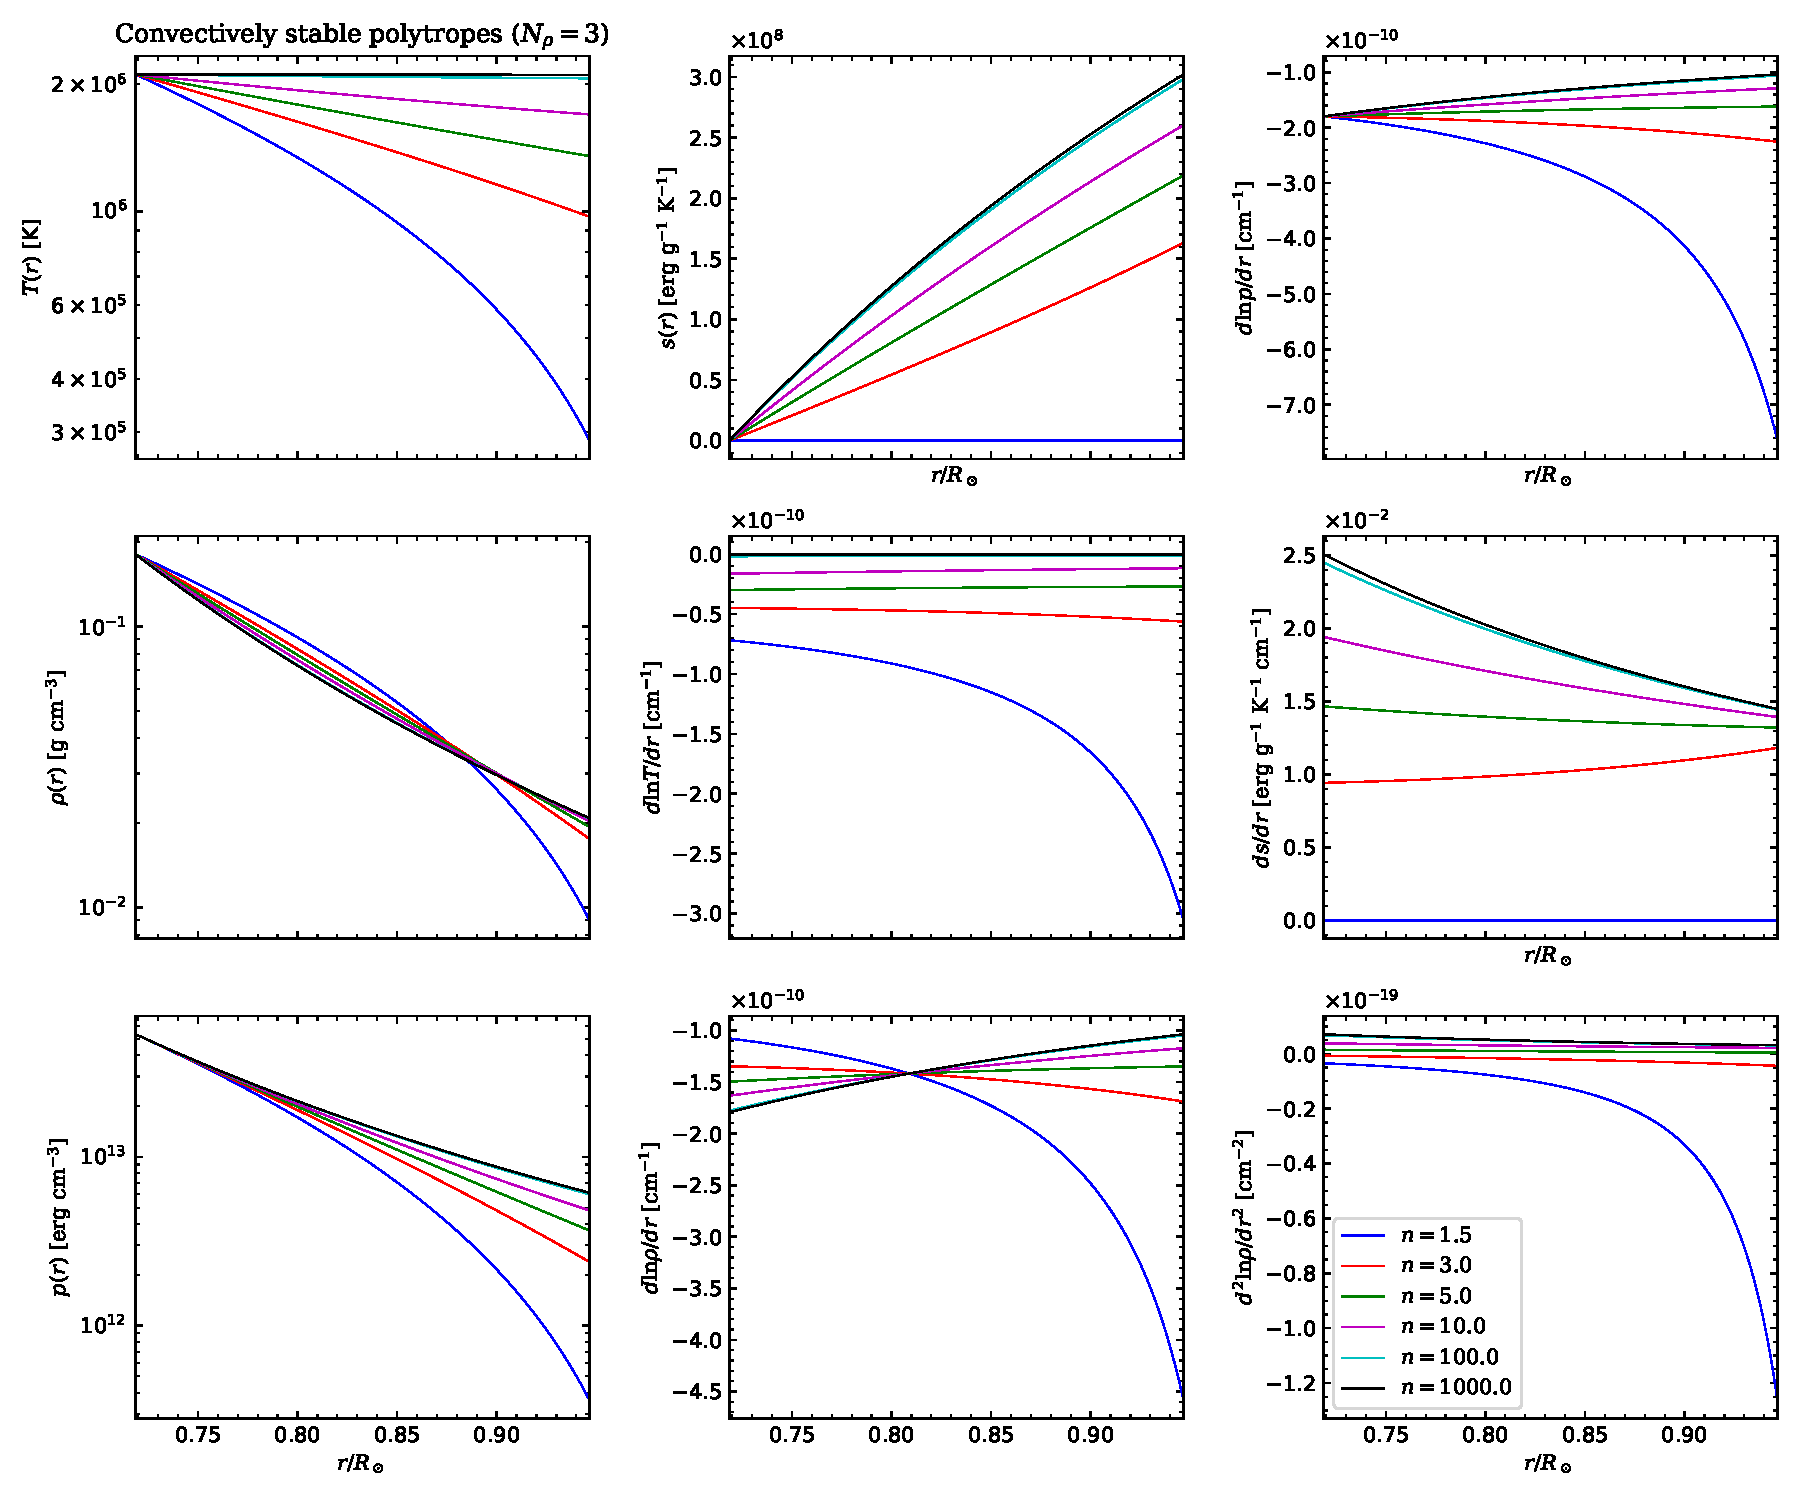
\includegraphics[scale=0.6]{figures/CZ_polytrope_stable.pdf}
	\caption{Sample of convectively stable polytropes for a solar-like CZ ($n\geq1.5$). The dimensional/geometric values for the polytrope (i.e., $\rm$, $r\topp$, $\rho\bcz$, $M$, $\cp$) are the solar values preceding \eqref{eq:kc_solar}, and $N_\rho=3$.}
	\label{fig:CZ_polytrope_stable}
\end{figure}

  \begin{figure}
	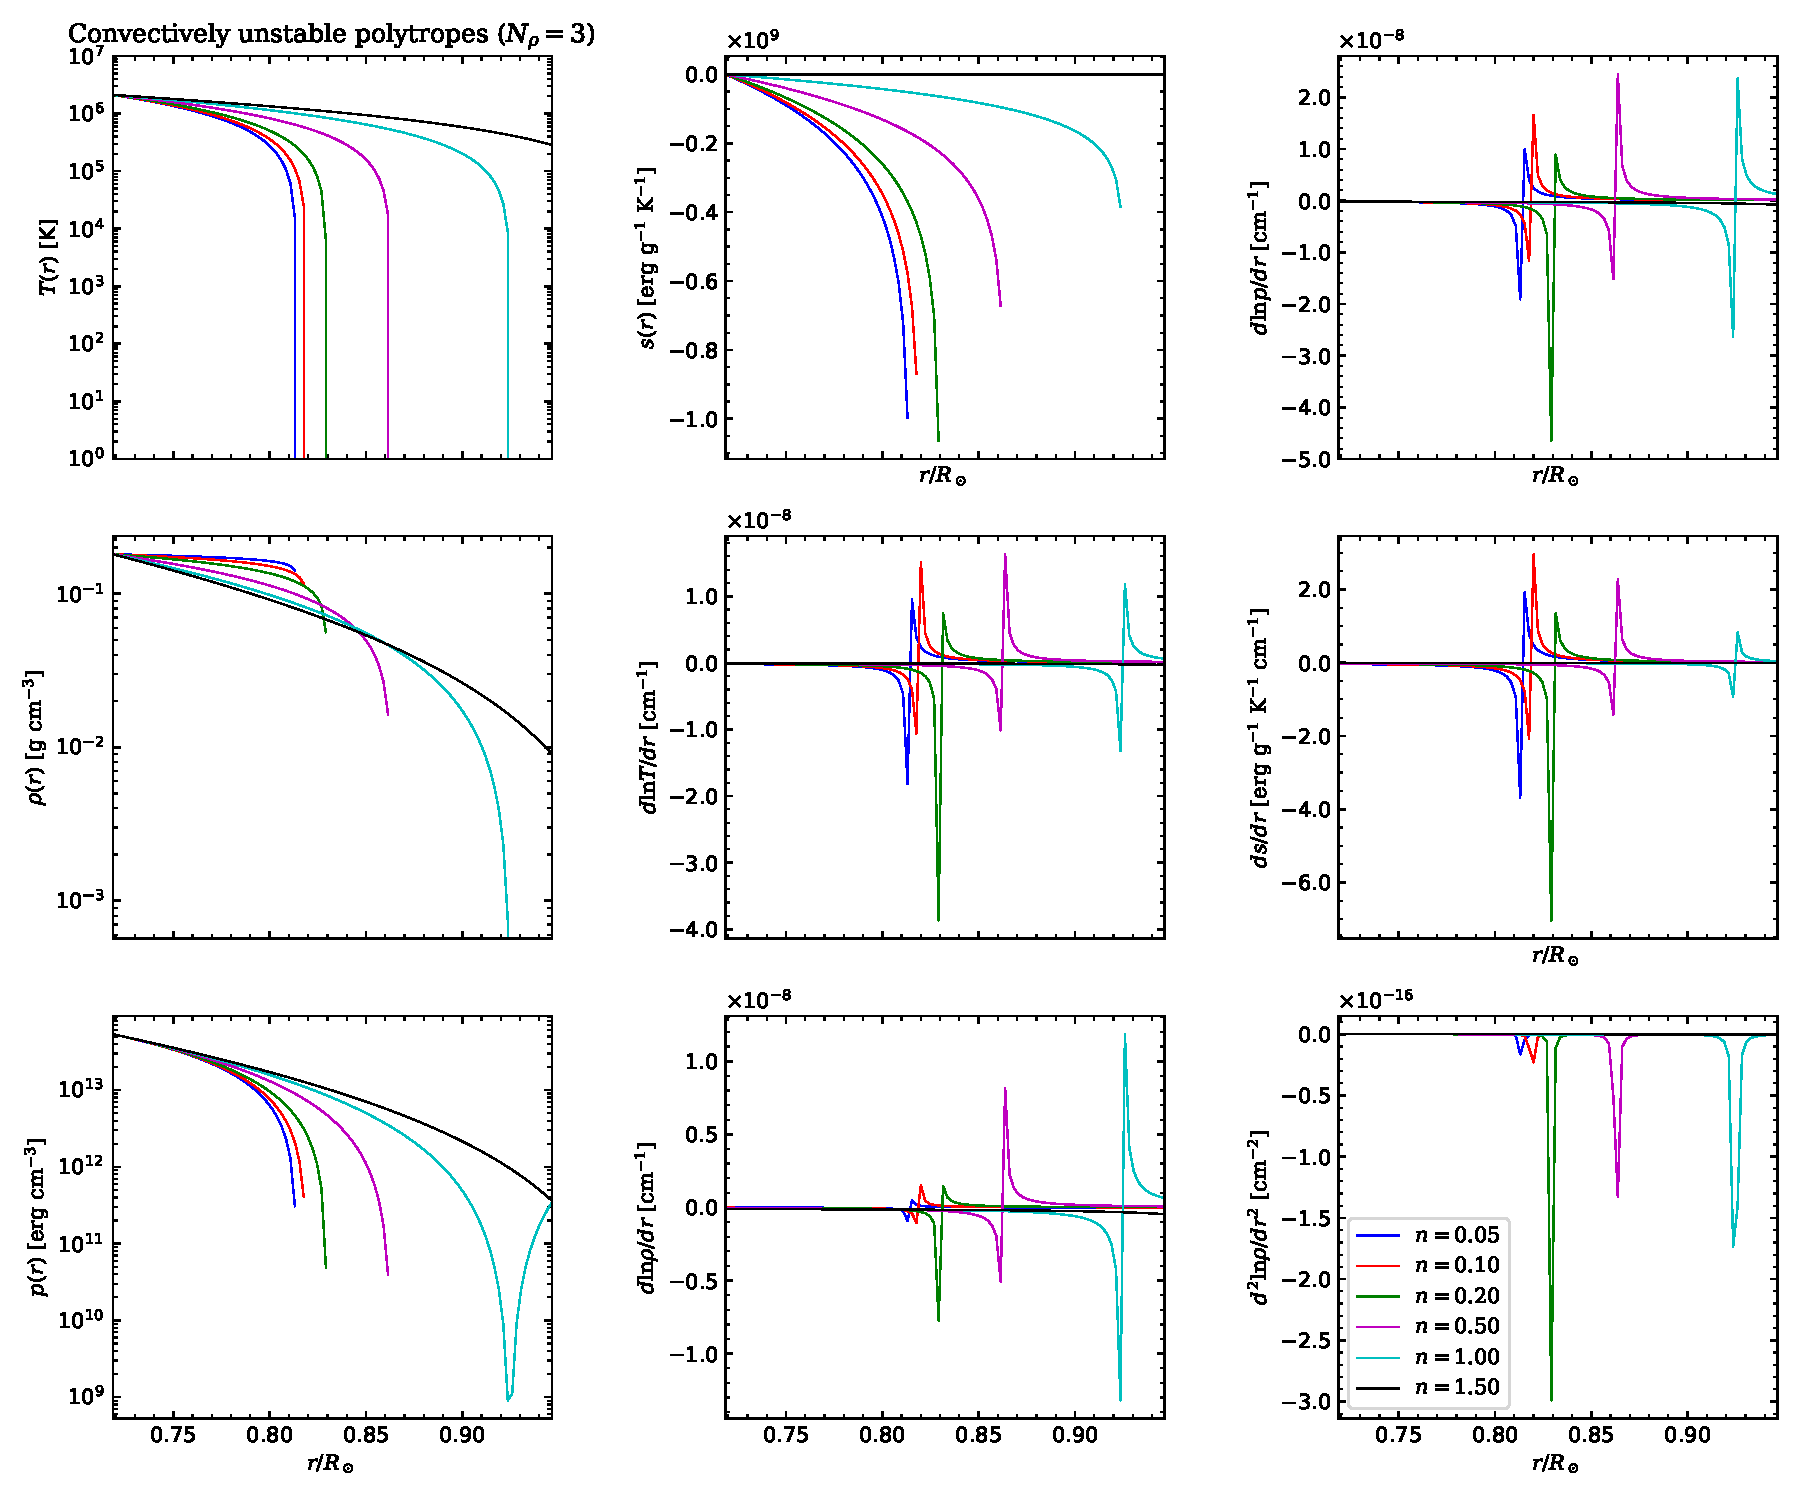
\includegraphics[scale=0.6]{figures/CZ_polytrope_unstable.pdf}
	\caption{Sample of convectively unstable polytropes for a solar-like CZ ($n\leq1.5$), with the same dimensional parameters as Figure \ref{fig:CZ_polytrope_stable}.}
	\label{fig:CZ_polytrope_unstable}
\end{figure}

  \begin{figure}
	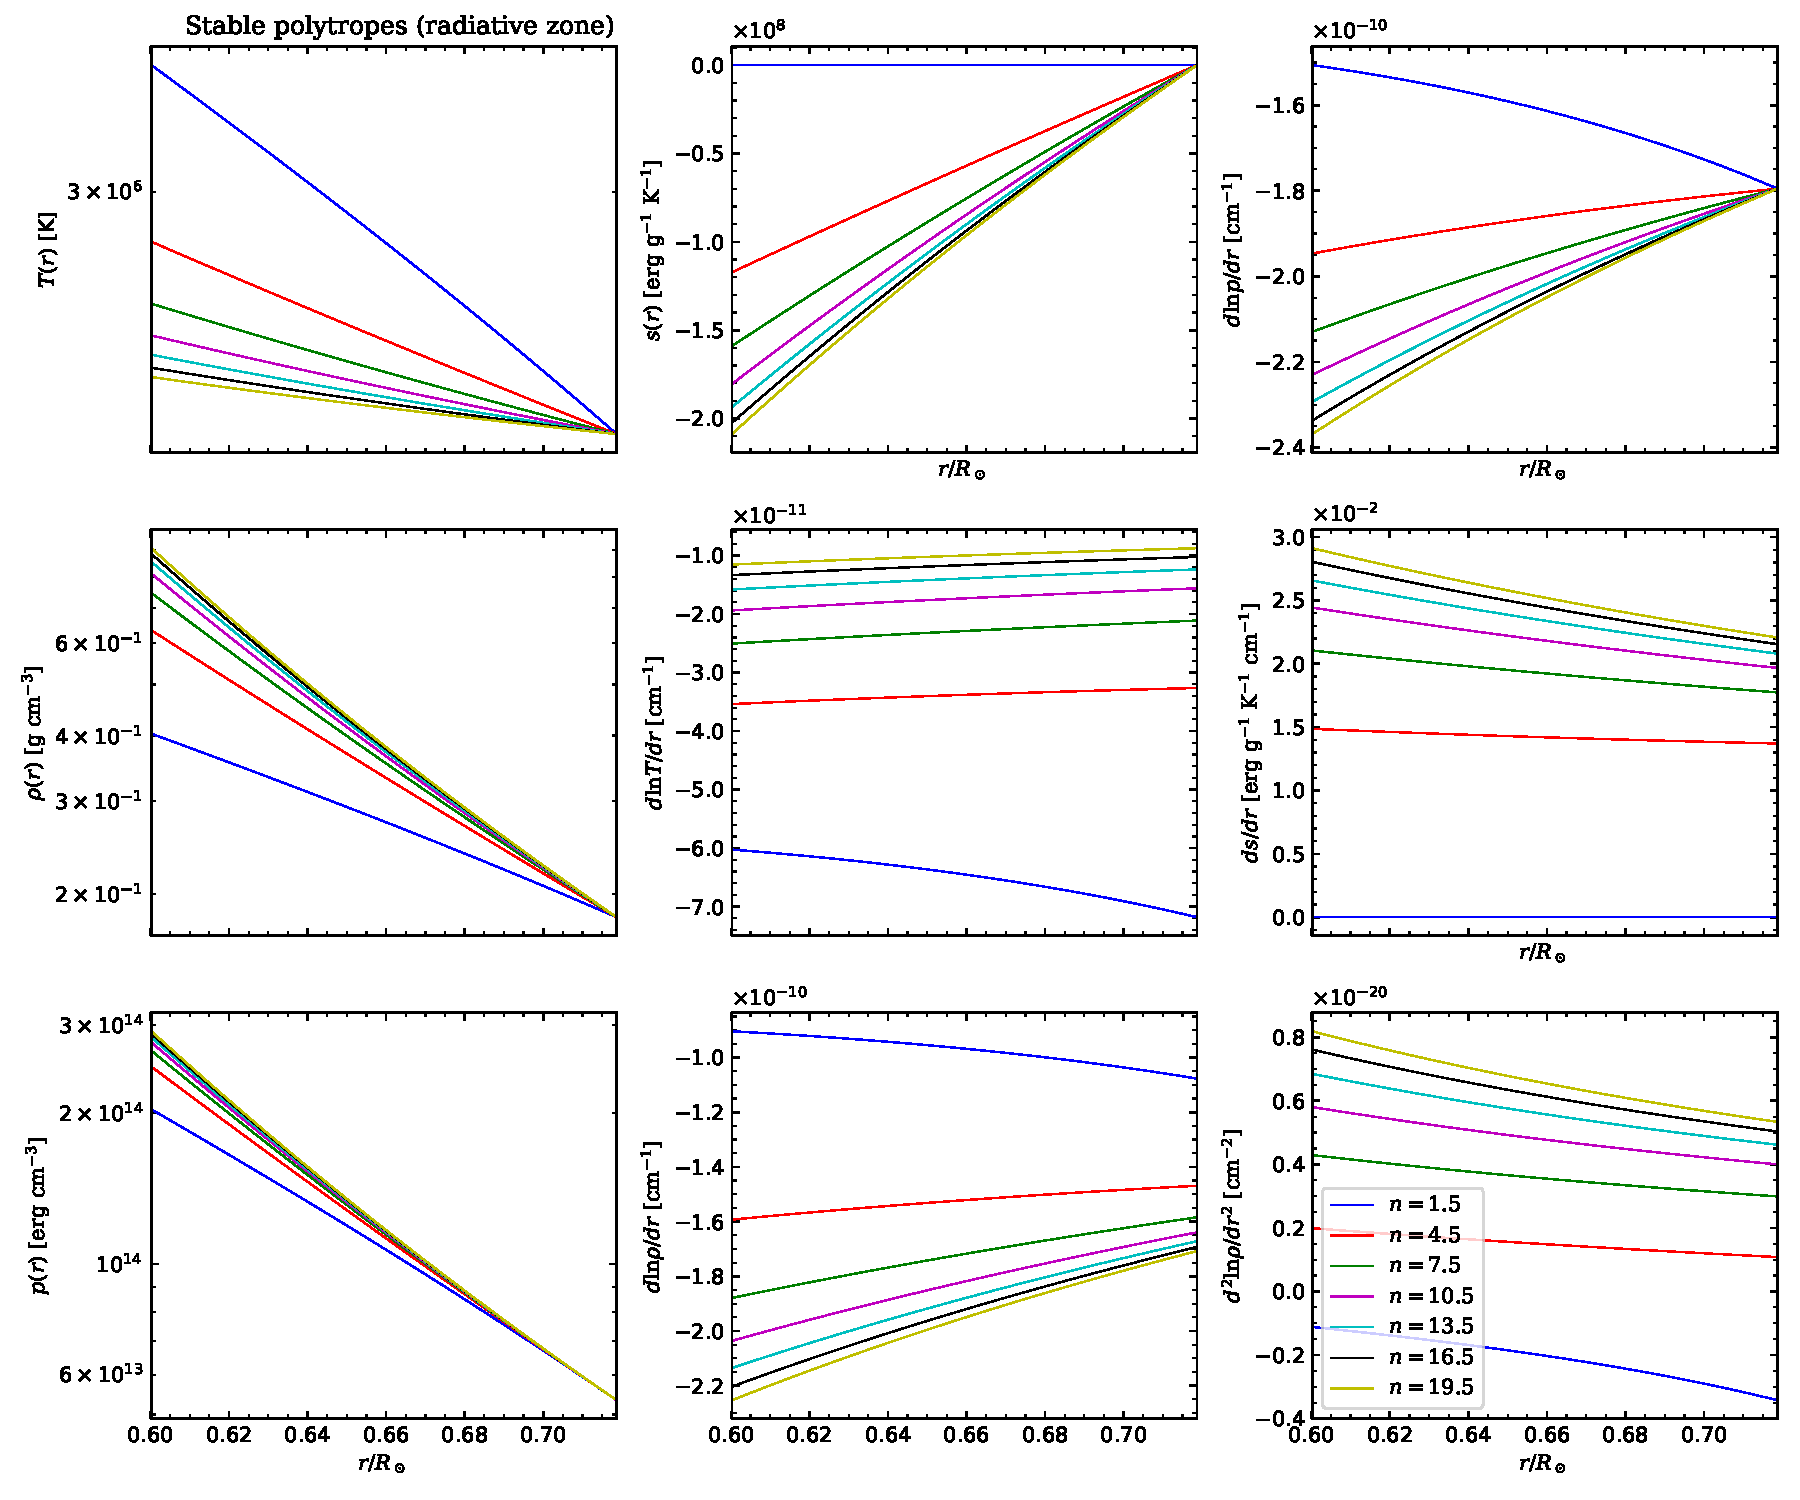
\includegraphics[scale=0.6]{figures/RZ_polytrope_stable.pdf}
	\caption{Sample of convectively stable polytropes for a solar-like RZ ($n\geq1.5$). Similar to Figure \ref{fig:CZ_polytrope_stable}, except the radius range is $(r\bott=4.176\times10^{10}\ {\rm{cm}},\ r\bcz=5.00\times10^{10}\ \rm{cm})$ instead of $(r\bcz,r\topp)$.}
	\label{fig:RZ_polytrope_stable}
\end{figure}

\begin{figure}
	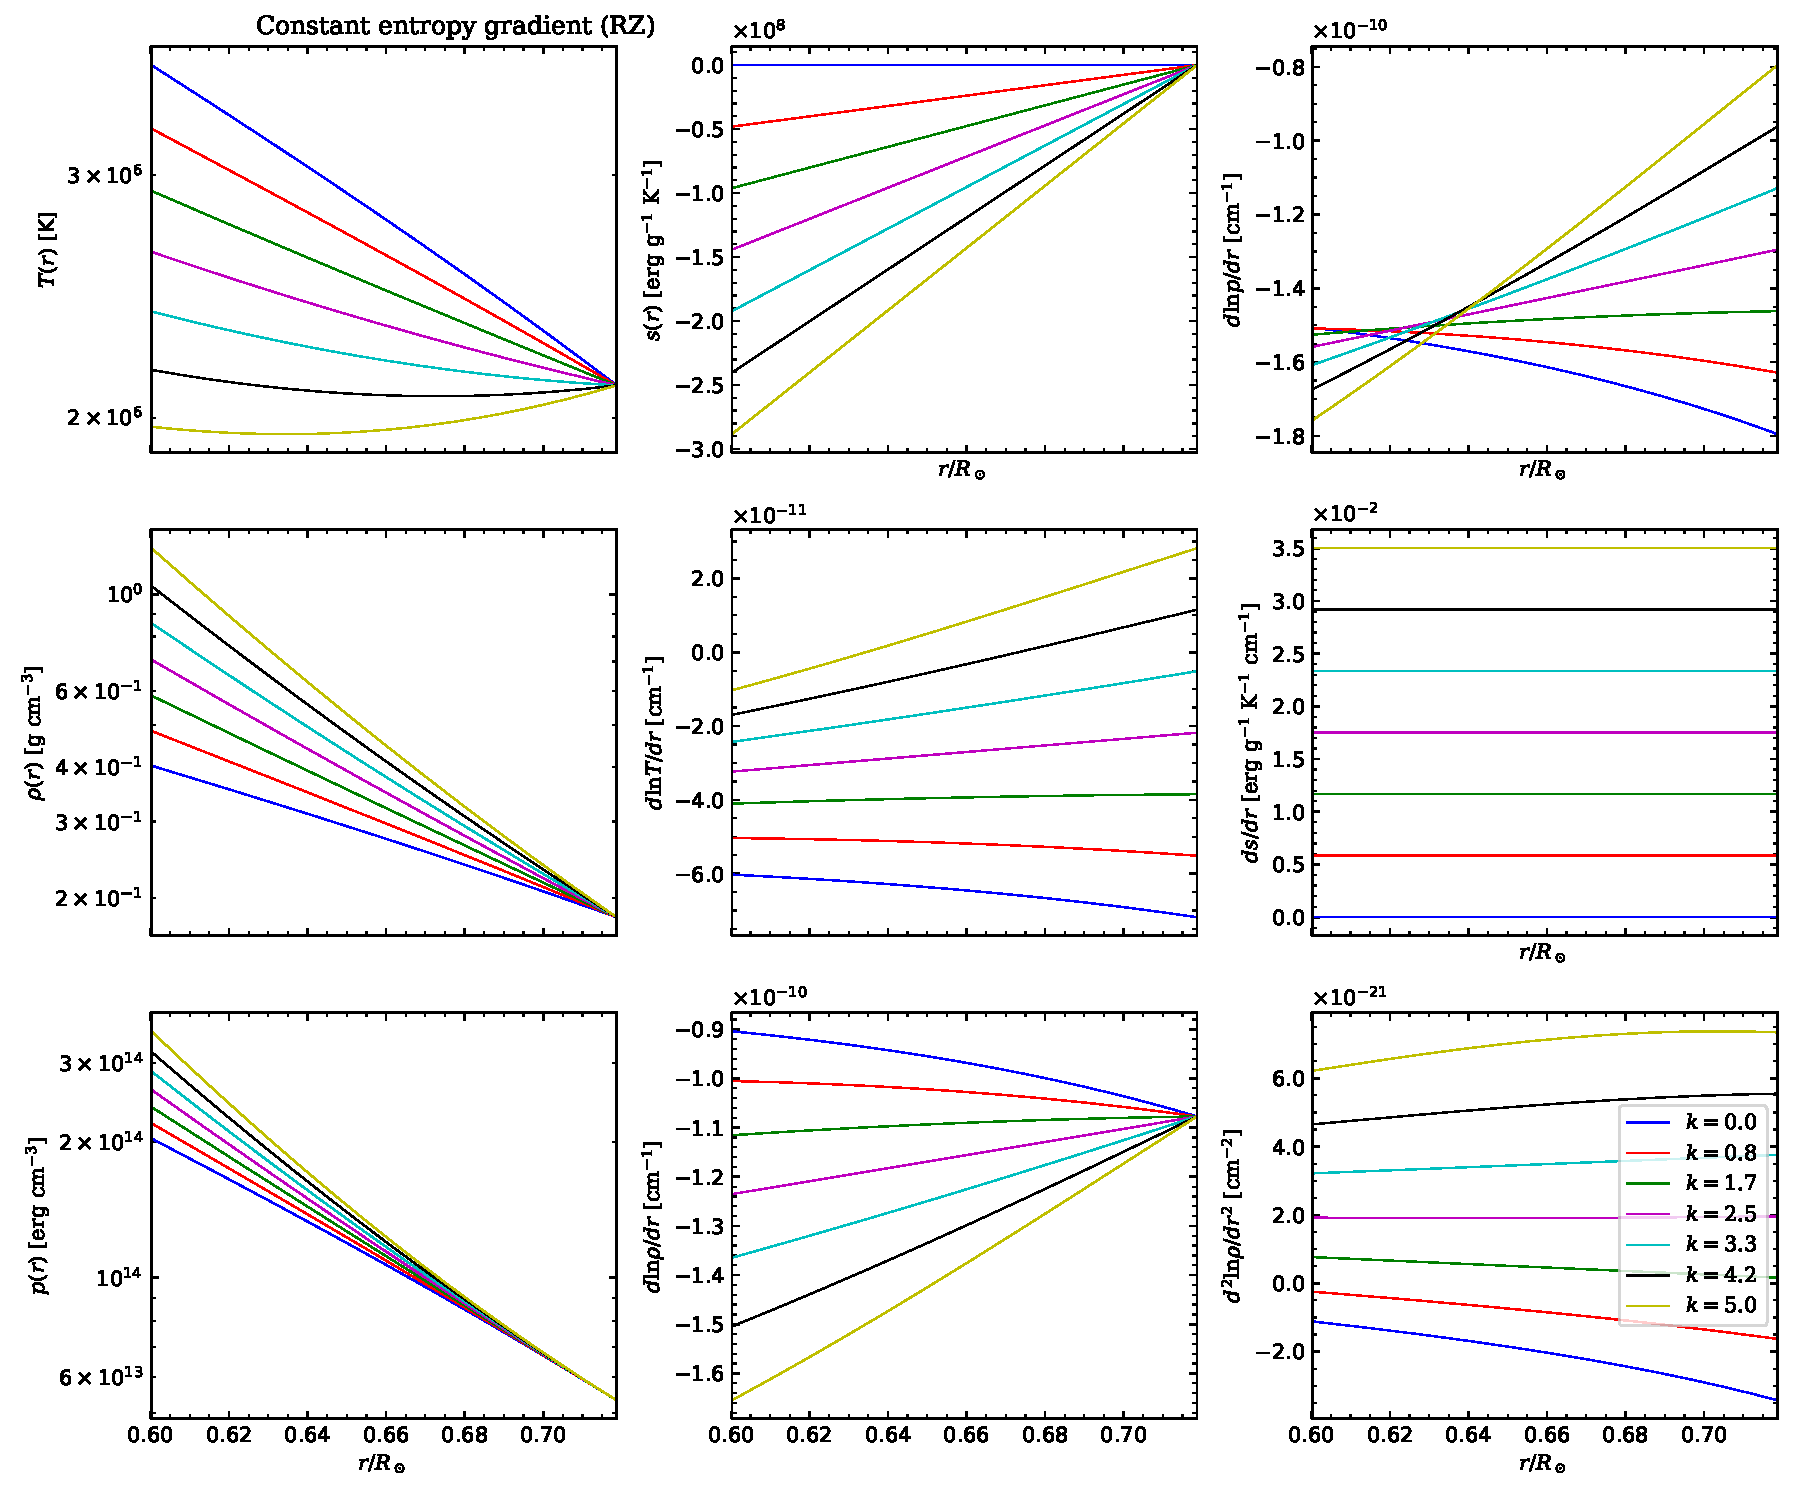
\includegraphics[scale=0.6]{figures/RZ_const_sgrad.pdf}
	\caption{Sample of constant-entropy-gradient gas layers for a solar-like RZ, with values of $k$ chosen to give entropy gradients more or less matching those of Figure \ref{fig:RZ_polytrope_stable}.}
	\label{fig:RZ_const_sgrad}
\end{figure}

\begin{figure}
	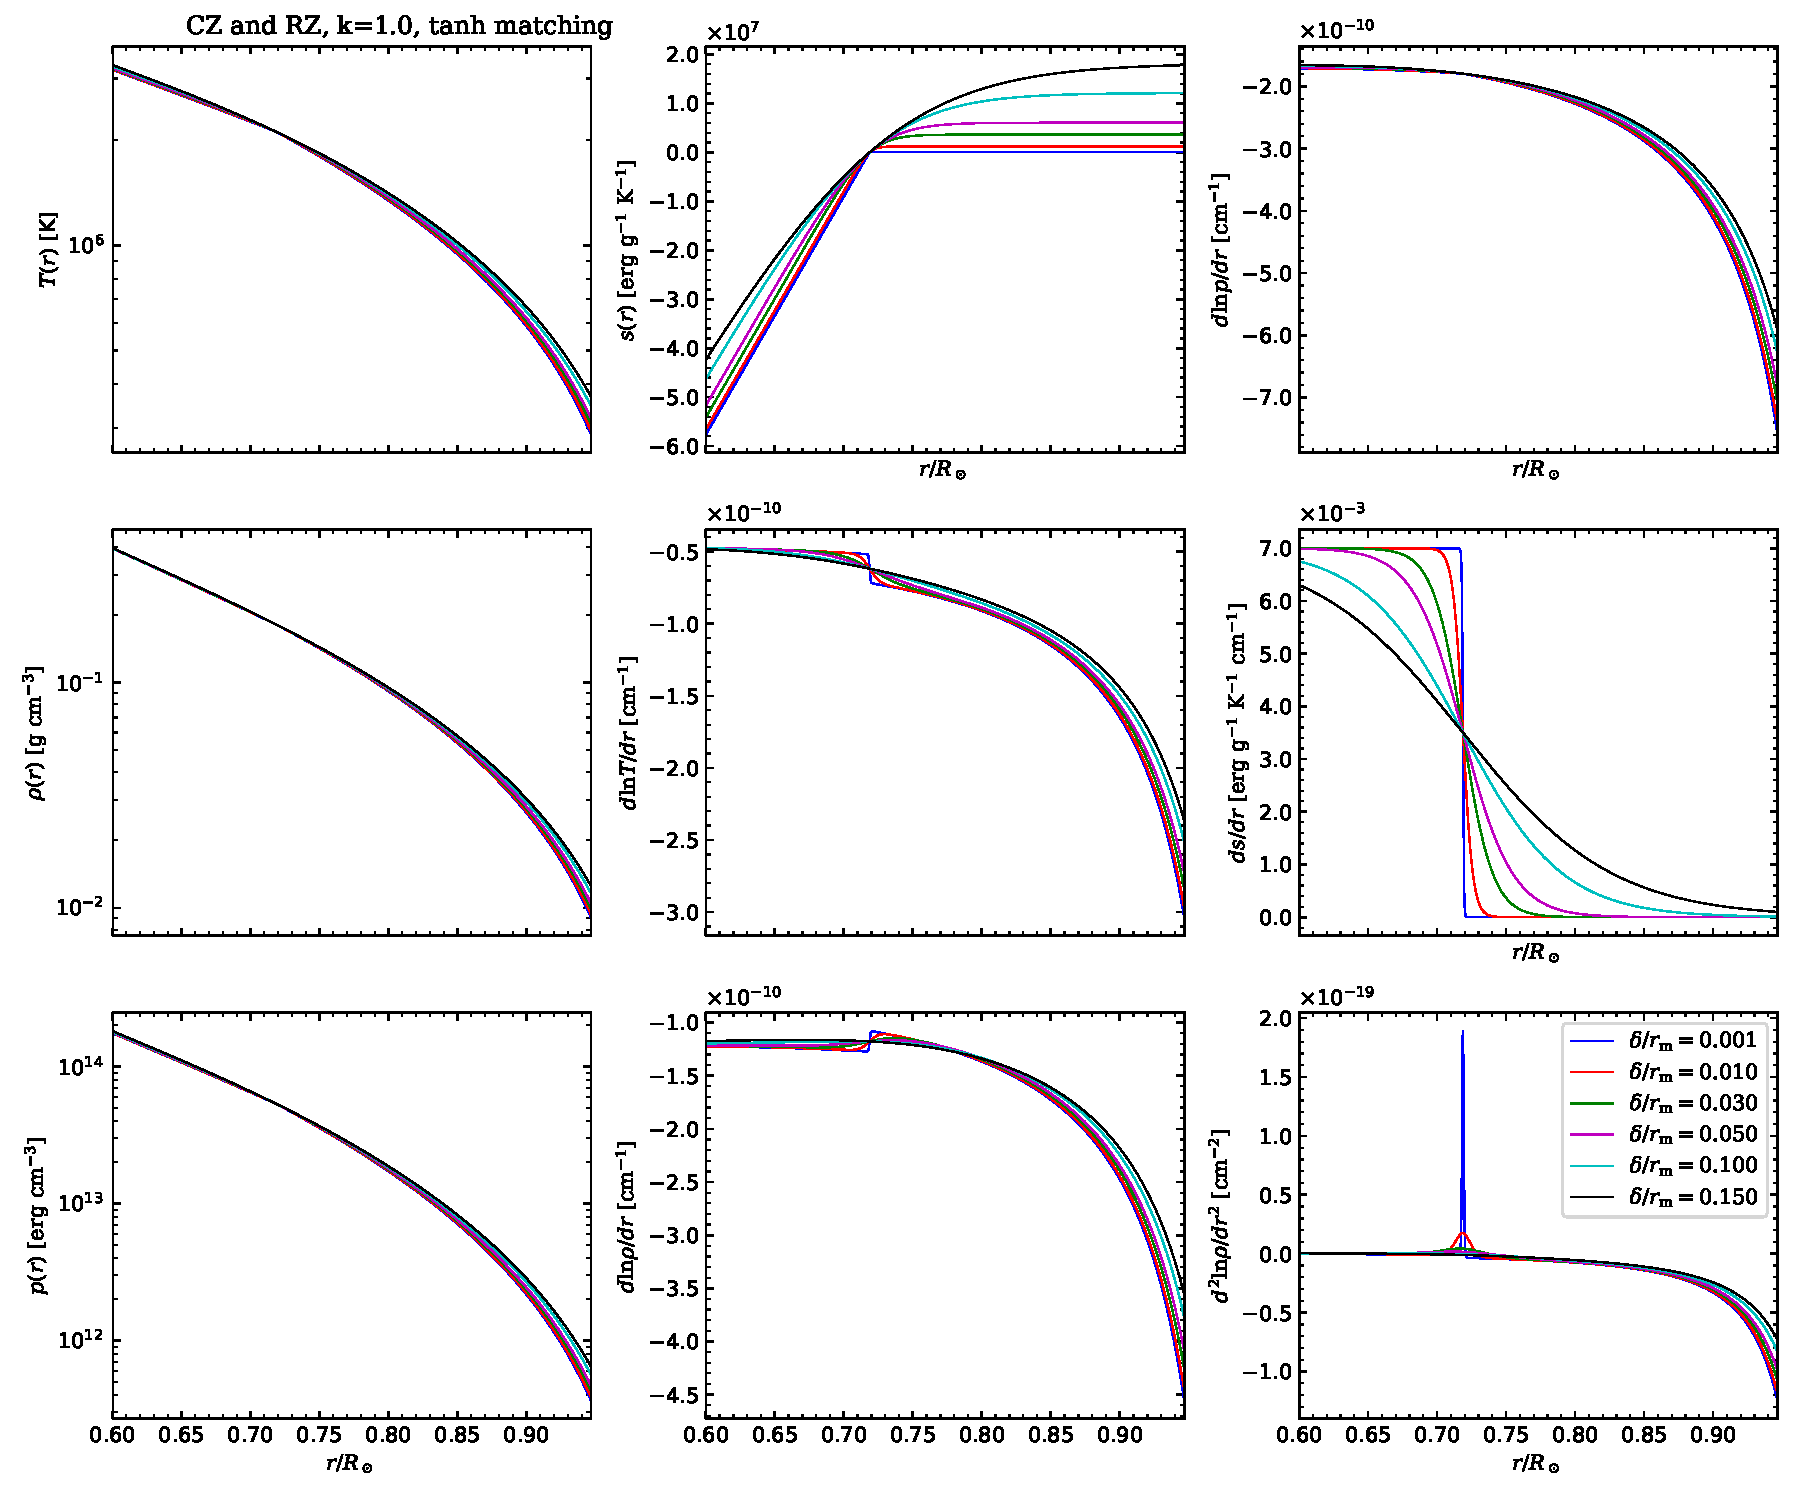
\includegraphics[scale=0.6]{figures/CZ_RZ_tanhmatch_vs_delta.pdf}
	\caption{Combined CZ and RZ fluid layer with entropy gradient profiles matched via hyperbolic tangents---different transition thicknesses $\delta$, with $k=1$ in all cases.}
	\label{fig:CZ_RZ_tanhmatch_vs_delta}
\end{figure}

\begin{figure}
	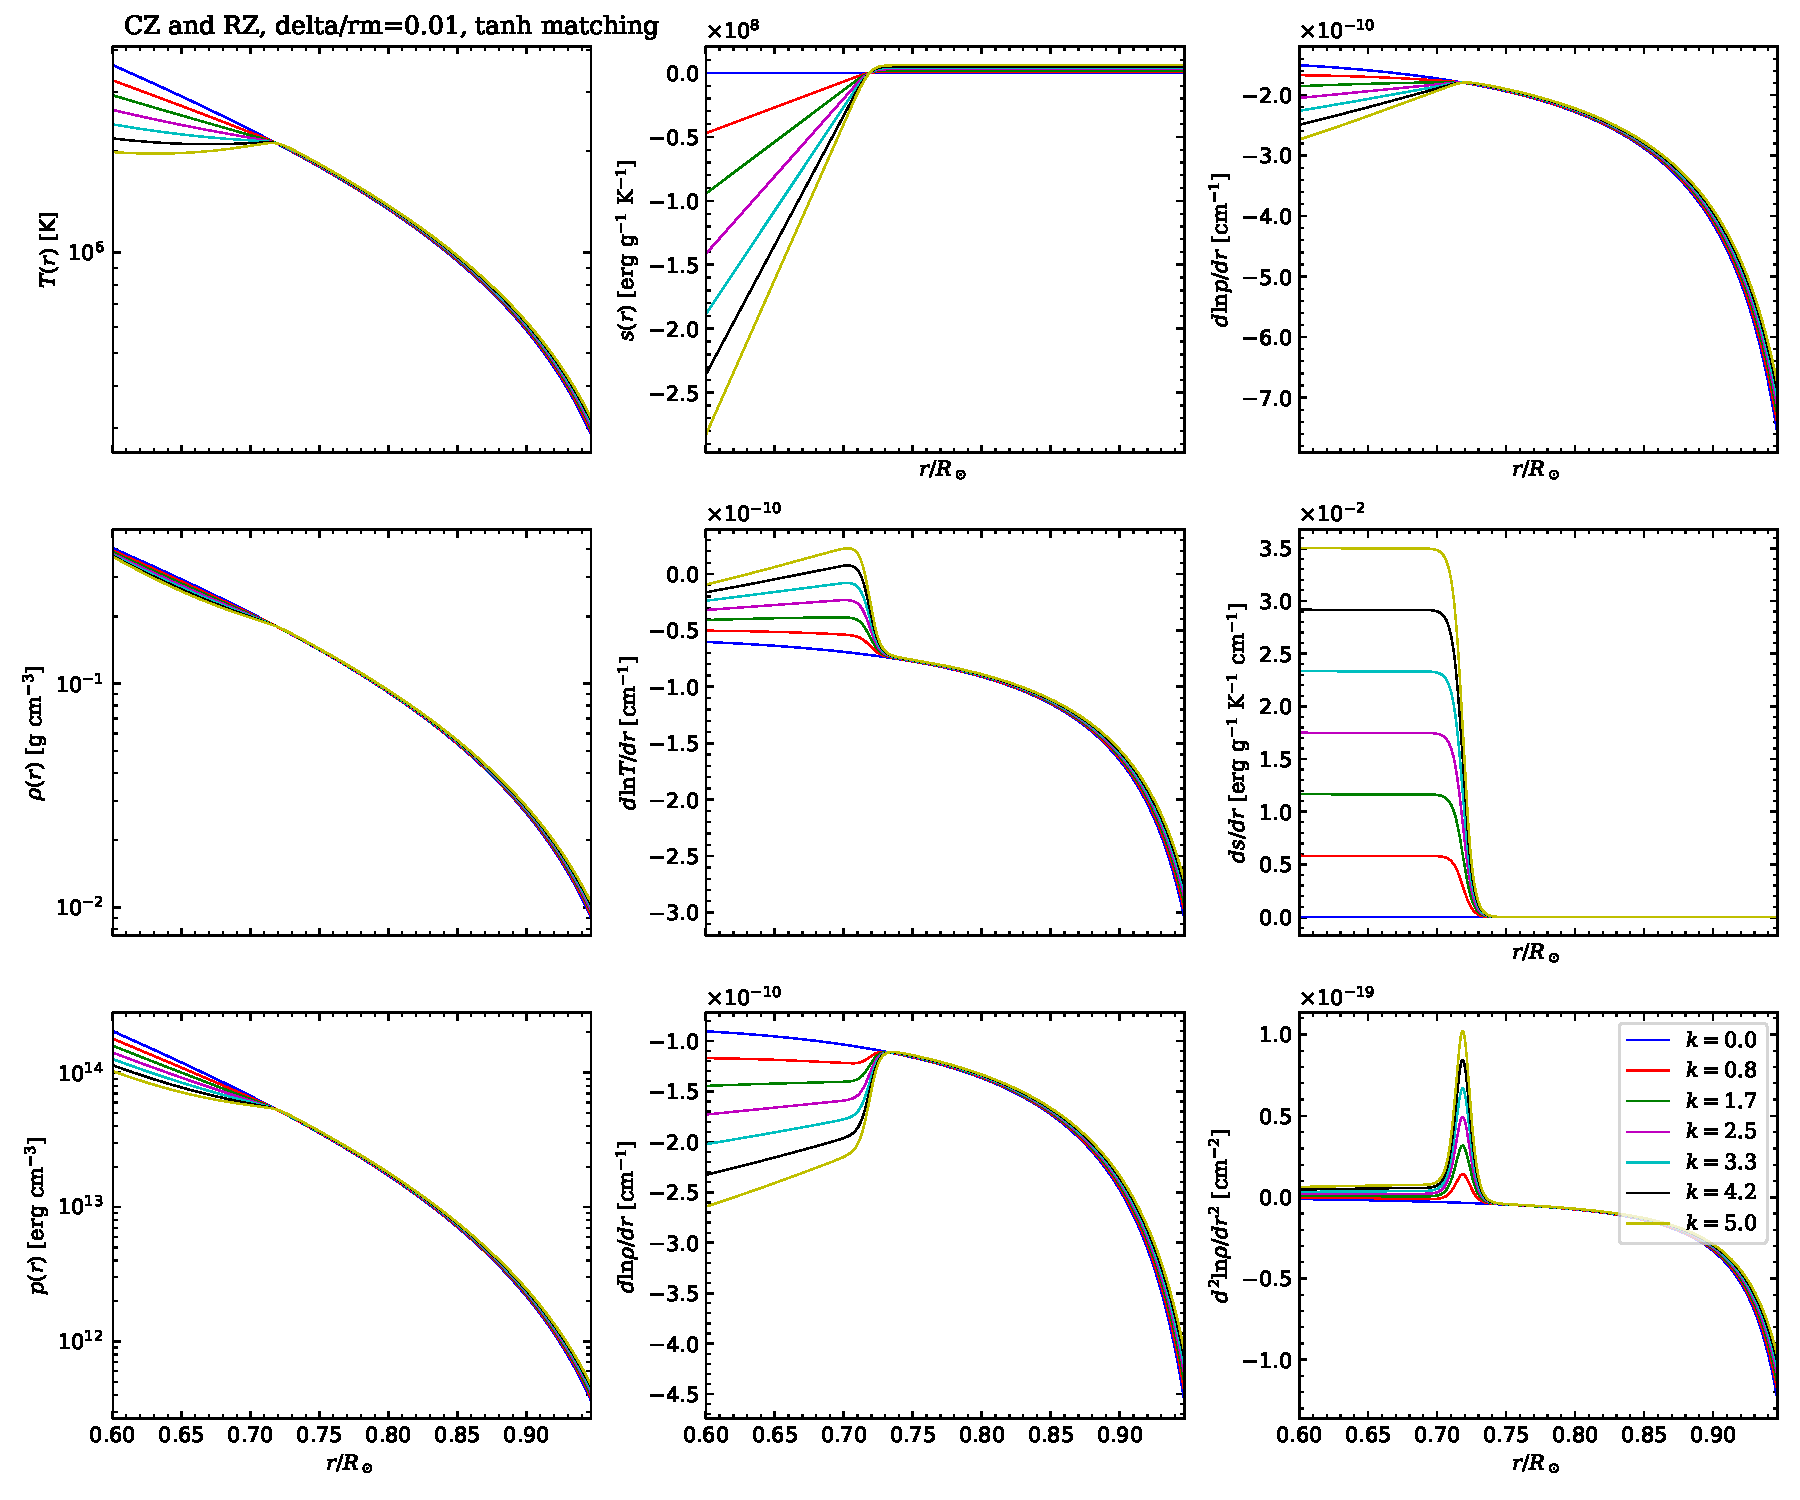
\includegraphics[scale=0.6]{figures/CZ_RZ_tanhmatch_vs_k.pdf}
	\caption{Combined CZ and RZ fluid layer with entropy gradient profiles matched via hyperbolic tangents---different levels of stiffness $k$, with $\delta/r\bcz=0.01$ in all cases.}
	\label{fig:CZ_RZ_tanhmatch_vs_k}
\end{figure}
\begin{figure}
	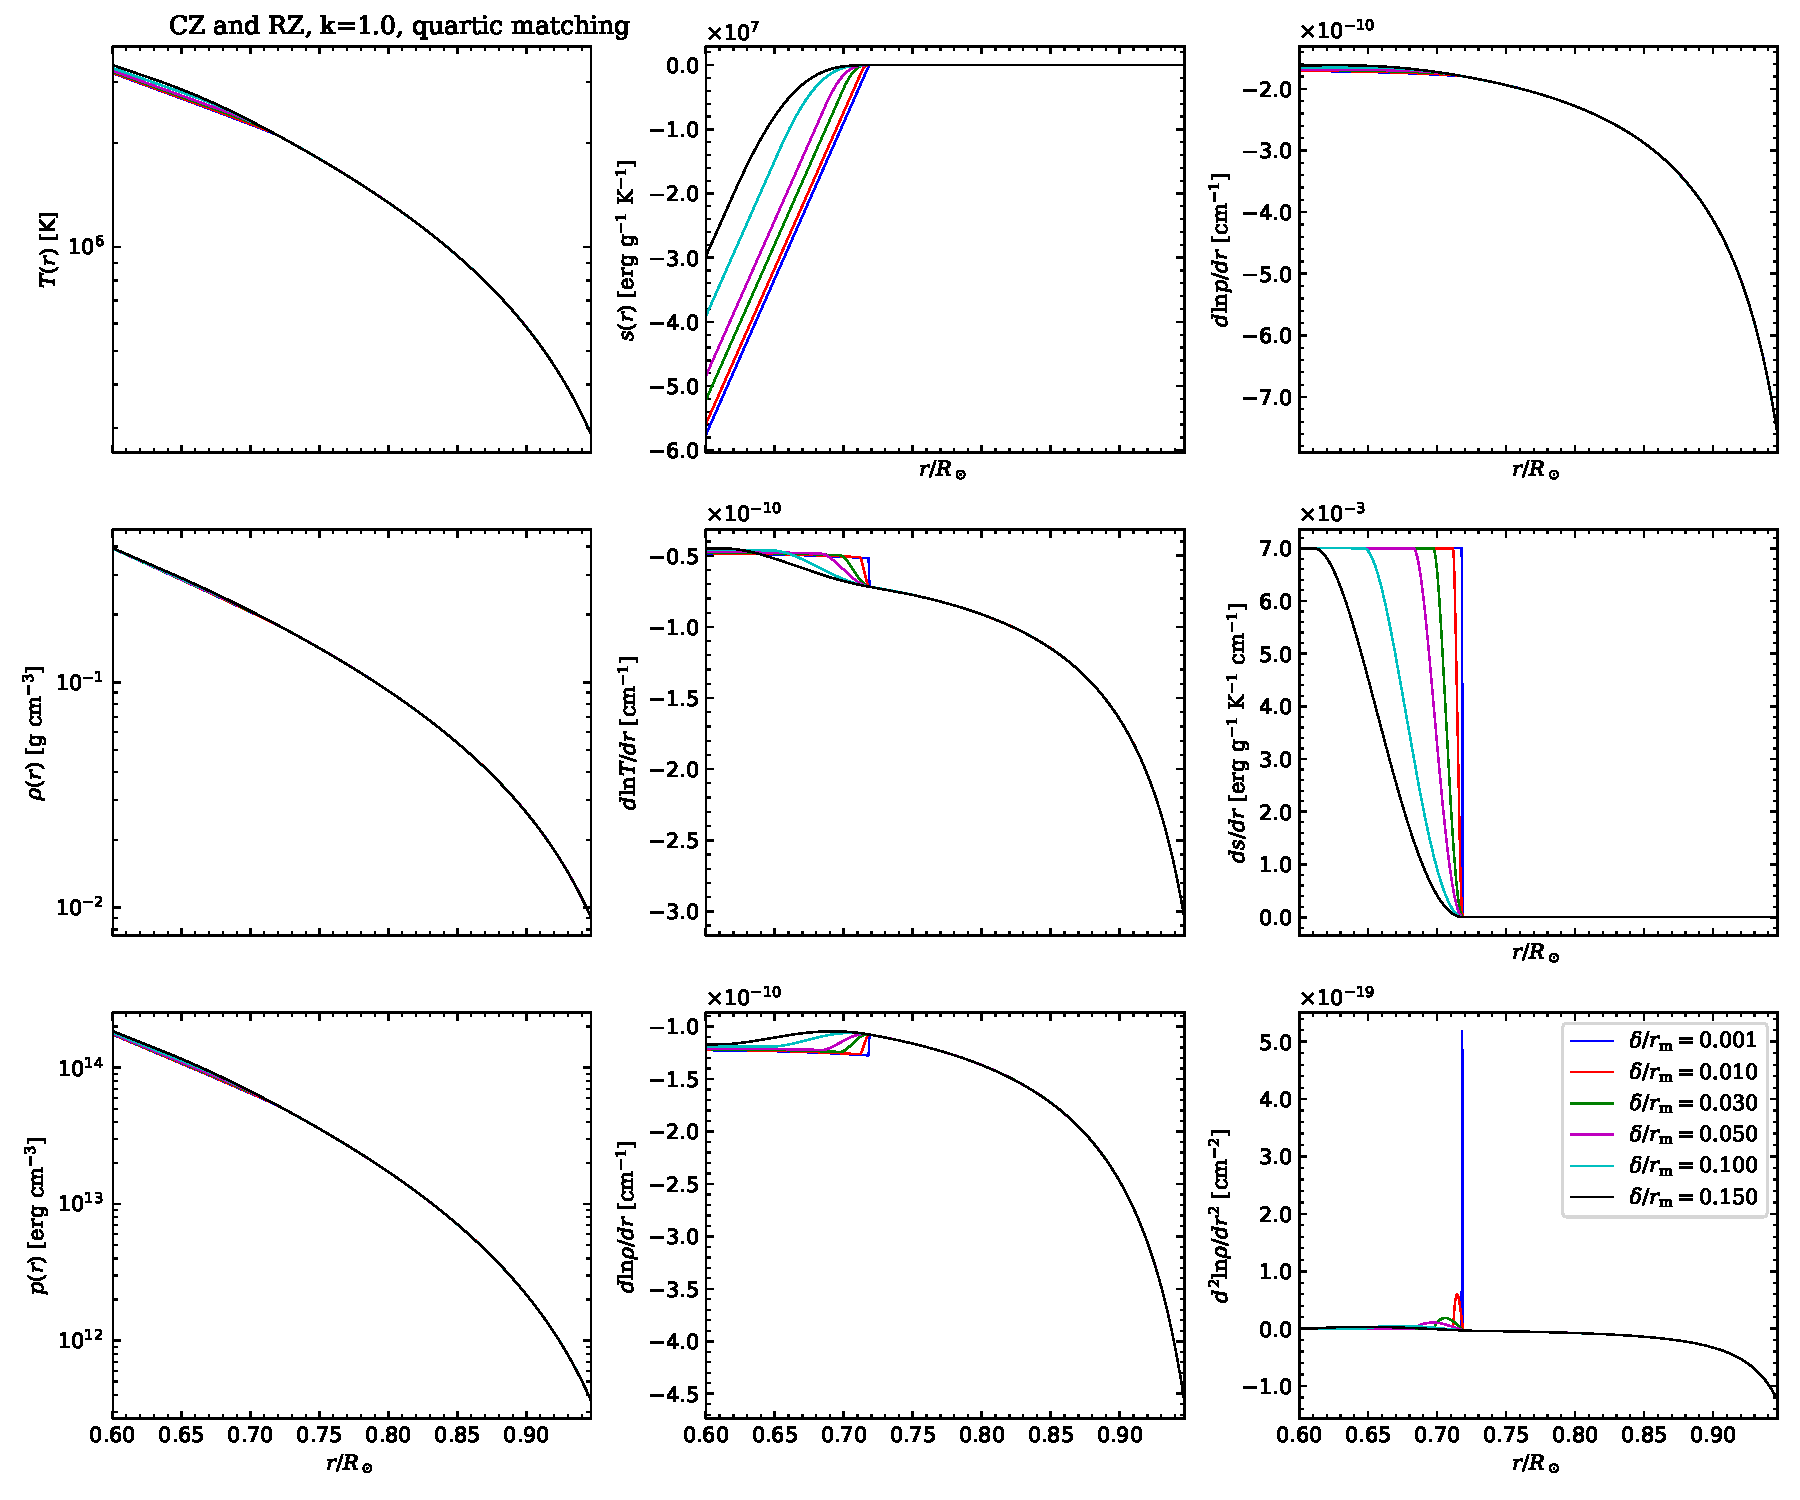
\includegraphics[scale=0.6]{figures/CZ_RZ_quartmatch_vs_delta.pdf}
	\caption{Combined CZ and RZ fluid layer with entropy gradient profiles matched via quartic functions---different transition thicknesses $\delta$, with $k=1$ in all cases.}
	\label{fig:CZ_RZ_quartmatch_vs_delta}
\end{figure}

\begin{figure}
	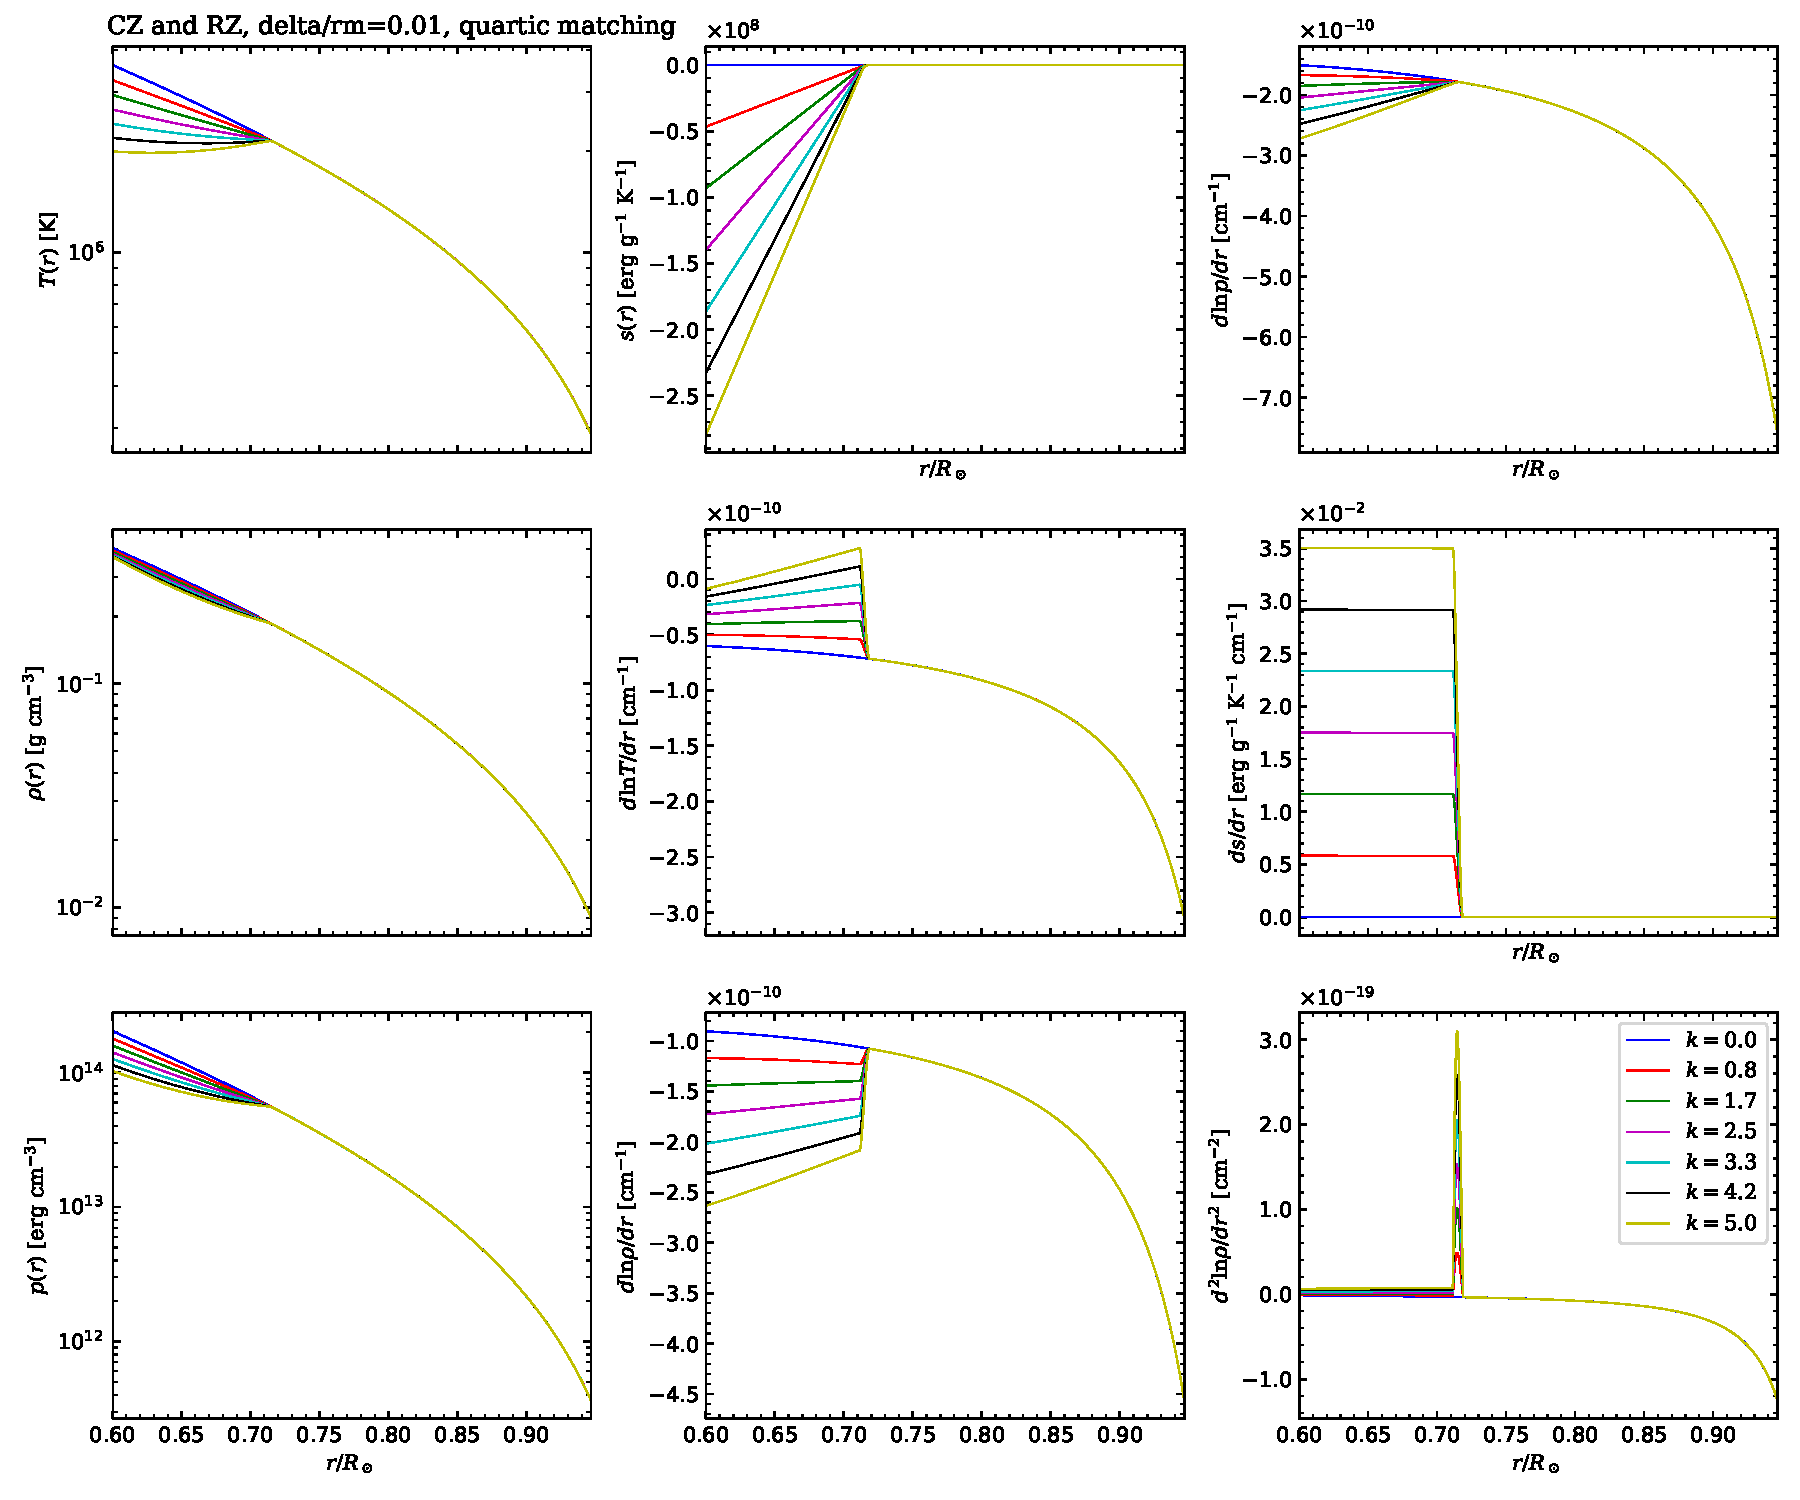
\includegraphics[scale=0.6]{figures/CZ_RZ_quartmatch_vs_k.pdf}
	\caption{Combined CZ and RZ fluid layer with entropy gradient profiles matched via quartic functions---different levels of stiffness $k$, with $\delta/r\bcz=0.01$ in all cases.}
	\label{fig:CZ_RZ_quartmatch_vs_k}	
\end{figure}
\end{document}